%!TEX TS-program = xelatex
%!TEX root = ../../maxwell2018thesis.tex

\chapter[Snippet Lengths and Stopping Behaviour]{Snippet Lengths and\\Stopping Behaviour}\label{chap:snippets}
Discussed previously in Section~\ref{sec:ir_background:user:iir:serp}, the~\glsfirst{acr:serp} is core to the experience of a searcher when utilising a retrieval system. The presentation and design of the~\gls{acr:serp} has over the years been subject to much research, but with more complex components (such as the \emph{information card}~\citep{navalpakkam2013non_linear_serp} or \emph{social annotations}~\citep{muralidharan2012social_annotations}) now becoming commonplace in contemporary web retrieval systems, much work still remains on examining how more traditional~\gls{acr:serp} components are designed and presented to searchers. \emph{Result summaries} are such a component.

\begin{figure}[h]
    \centering
    \vspace{4mm}
    \resizebox{1\hsize}{!}{
    
\includegraphics{figures/ch7-serpintro.pdf}}
    \label{fig:serpintro}
    \vspace{-5mm}
\end{figure}

These summaries (an example of which is shown above) have been traditionally viewed as the \emph{ten blue links}, each with their corresponding title and source (typically a~\gls{acr:url}) of the document. Included with these two components are the textual \emph{snippets} of \emph{keywords-in-context}, derived from the document itself. These snippets are approximately 130-150 characters (or two lines) in length~\citep{hearst2009_search}. Numerous researchers have explored result summaries in a variety of different ways, such as: examining their length~\citep{paek2004wavelens,cutrell2007eye_tracking,kaisser2008improving}; the use of thumbnails~\citep{woodruff2002summaries,teevan2009visual_snippets}; their attractiveness~\citep{clarke2007caption_features,he2012bridging}; and the generation of \emph{query-biased snippets}~\citep{tombros1998query_biased,rose2007snippet_attributes}. In essence, the length of result summaries presented to searchers has been shown to influence the point at which they stop examining the content provided in a ranked list of results. 

% The performance of searchers has broadly been evaluated in a limited fashion (for example, by examining task completion times). 

In this chapter, we are interested in examining how the length (and subsequently information content) of result summaries affects~\gls{acr:serp} interactions -- specifically examining their stopping behaviours -- and a searcher's ability to select relevant over non-relevant items. This is in tandem with an examination of different stopping strategies (outlined in Chapter~\ref{chap:strategies}), and how they adapt to increasing snippet lengths. Prior research has demonstrated that longer result summaries tend to lower completion times for informational tasks, where searchers need to find only a single relevant document~\citep{cutrell2007eye_tracking}. Does this finding however hold in an ad-hoc context, where searchers need to find \emph{several} relevant items? Furthermore, how does the length and information associated with longer result summaries affect the searcher's ability to discern the relevant from the non-relevant? We address these questions from the perspective of both:

\begin{itemize}
    \item{a \blueboxbold{user study} examining this phenomenon, as detailed in Section~\ref{chap:snippets:user}; and}
    \item{a \blueboxbold{simulated analysis}, closely examining how varying snippet lengths affects searcher performance and stopping behaviours, discussed in Section~\ref{sec:snippets:simulations}.}
\end{itemize}

The outline for both of these studies follow the general methodology, as discussed in Chapter~\ref{chap:method}. Before discussing the studies and their results, we begin this chapter with an overview of the prior work that has examined the length of result summary snippets.

\section{Background}\label{chap:snippets:background}
As previously discussed, the design and presentation of~\glsplural{acr:serp} has been examined in depth. Researchers have examined various aspects of~\glsplural{acr:serp}, and how the designs of such aspects influence the behaviour of searchers. In this section, we provide a summary of the various aspects that have been examined over time. Specifically, we consider:

\begin{itemize}
    \item{the layout and presentation of~\glsplural{acr:serp};}
    \item{the size of~\glsplural{acr:serp};}
    \item{how snippet text for result summaries is generated; and}
    \item{how much text should be presented within each result summary}.
\end{itemize}

Of the four areas of~\gls{acr:serp} research that we examine in this section, we consider the latter to be the main focus of this work. Each area is summarised below.

\subsection{SERP Layout and Presentation}
Early works regarding the presentation of result summaries examined different approaches to automatically categorising result summaries for searchers, similar to the categorisation approach employed by early search engines (as shown in Figure~\ref{fig:yahoo} on page~\pageref{fig:yahoo}). ~\cite{chen2000order_to_web} developed an experimental system that automatically categorised result summaries on-the-fly as they were generated. For a query, associated categories were then listed as verticals, with associated document titles provided underneath each category header. Traditional result summaries were then made available when hovering over a document title. Subjects of a user study found the interface easier to use than the traditional \emph{ten blue links} approach -- they were 50\% faster at finding information displayed in categories. This work was then extended by~\cite{dumais2001results_in_context}, where they explored the use of hover text to present additional details about search results based upon user interaction. Searching was also found to be slower with hover text, perhaps due to the fact that searchers were required to consider decision about when to seek additional information explicitly.

Alternatives to the traditional, linear list of result summaries have also been trialled (like grid-based layouts~\citep{resnick2001modeling, kammerer2010interface, chierichetti2011two_dimensional_presentation}). For example,~\cite{kammerer2010interface} examined differences in searcher behaviour when interacting with a standard list interface, compared against a tabular interface (title, snippet and~\gls{acr:url} stacked horizontally in three columns for each result), and a grid-based layout (result summaries placed in three columns). Those using the grid layout spent more time examining result summaries, and demonstrated promise in overcoming issues such as \emph{position bias}~\citep{craswell2008click_models}, as observed by~\cite{joachims2005click_model}.

\cite{marcos2015snippets_web_search} also performed an eye-tracking user study examining the effect of searcher behaviour while interacting with~\glsplural{acr:serp} -- and whether the \emph{richness} of result summaries provided on a~\gls{acr:serp} (i.e. result summaries enriched with metadata from corresponding pages) impacted upon the user's search experience. Enriched summaries were found to help capture a searcher's attention. Including both textual and visual representations of a document when presenting results could have a positive effect on relevance assessment and query reformulation~\citep{joho2006presentation}. Enriched summaries were also examined by~\cite{ali2009interaction_interfaces} in the context of navigational tasks. Striking a good balance between textual and visual cues (i.e. \emph{proximal cues,} as discussed in Section~\ref{sec:stopping_background:theoretical:ift:patch}) were shown to better support a searcher's tasks, and search completion time.

\subsection{Generating Snippet Text}
Searchers can be provided with an insight by result summaries as to whether a document is likely to be relevant or not~\cite{he2012bridging}. Consequently, research has been undertaken that examined different kinds of snippets, and how long a snippet should be. Work initially focused upon how these summaries should be generated~\citep{pedersen1991snippet, landauer1993enhancing, tombros1998query_biased, white2003task, leal2015query}. These early works proposed the idea of summarising documents with respect to the query (query-biased summaries), or keywords-in-context -- as opposed to simply extracting the representative or lead sentences from the document~\citep{kupiec1995tds}. Examples of both approaches are illustrated in Figure~\ref{fig:snippet_types}. Indeed,~\cite{tombros1998query_biased} showed that subjects of their study were likely to identify relevant documents more accurately when using query-biased summaries, compared to summaries that were simply generated from the first few sentences of a given document. Query-biased summaries have also been more recently shown to be preferred on mobile devices, too~\citep{spirin2016snippets}.

\begin{figure}[t!]
    \centering
    \resizebox{1\hsize}{!}{
    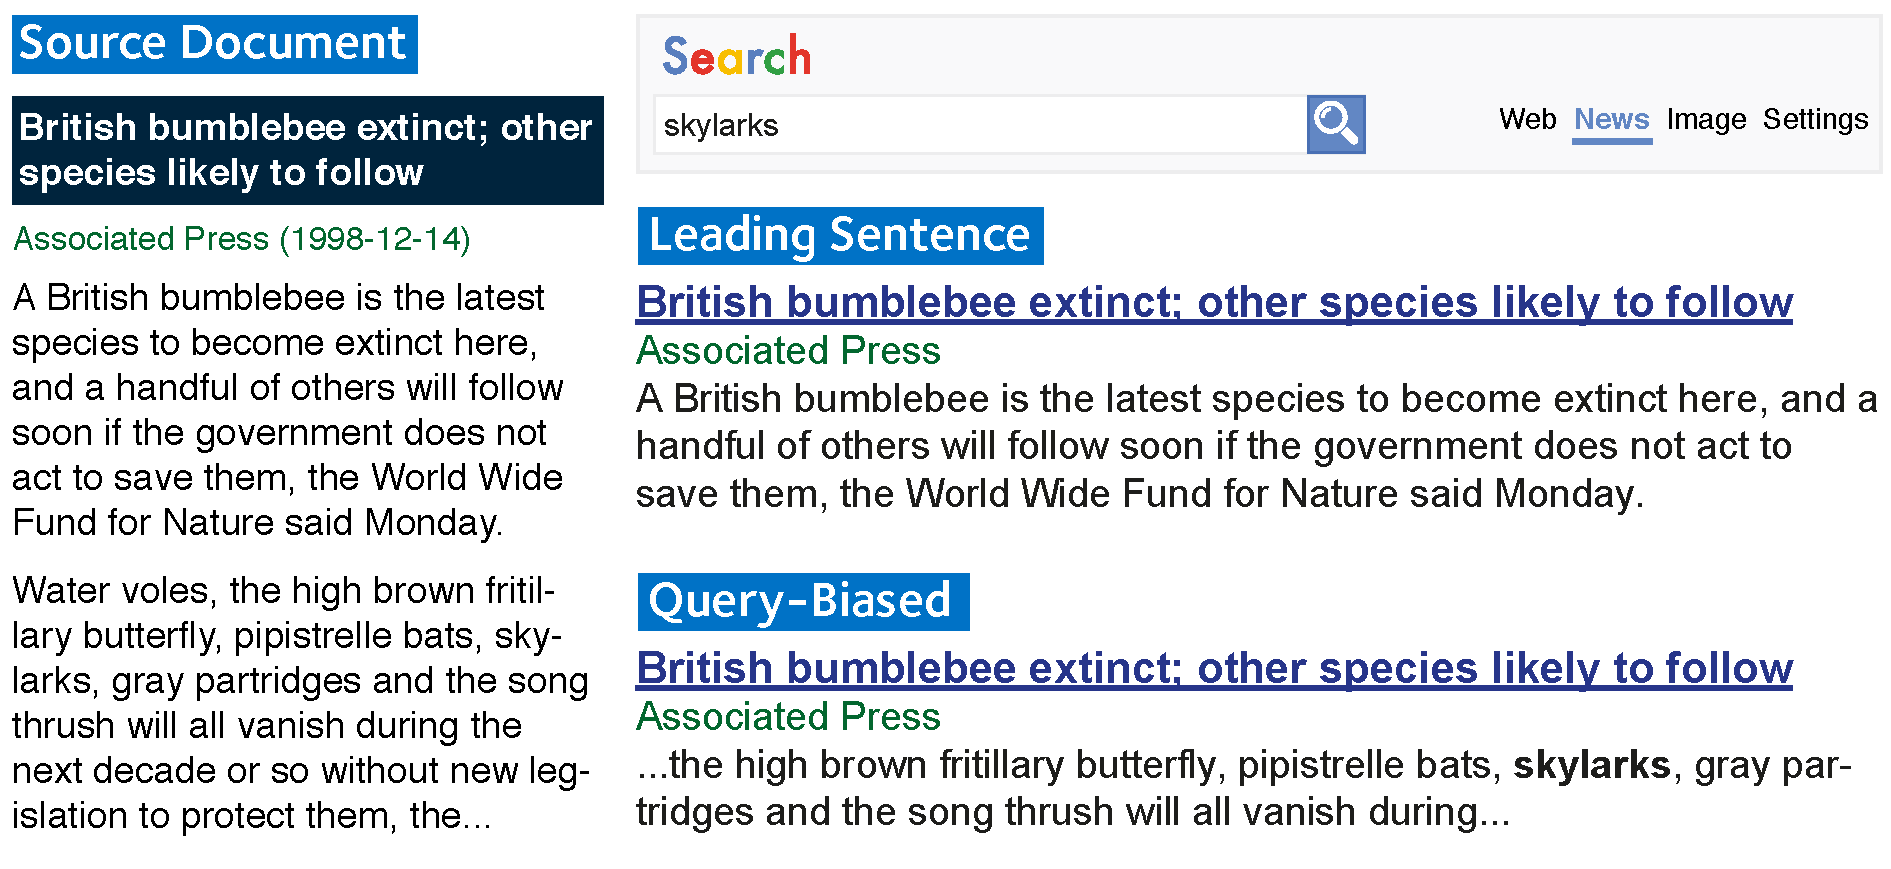
\includegraphics{figures/ch7-snippet_types.pdf}}
    \caption[Leading sentence and query-biased summary examples]{A visual example of two different types of summary, along with a portion of an example document from the~\gls{acr:trec} AQUAINT collection. Given the query \texttt{skylarks}, the \searchlogo~result summaries for both leading sentence and query-biased summaries are shown. Note the highlighting of the term \textbf{skylarks} in the query-biased summary.}
    \label{fig:snippet_types}
\end{figure}

When constructing snippets using query-biased summaries,~\cite{rose2007snippet_attributes} found that a user's perceptions of the result's quality were influences by the snippets. If snippets contained truncated sentences or many fragmented sentences (denoted as \emph{text choppiness}), searchers perceived the quality of the results more negatively, regardless of length.~\cite{kanungo2009snippet_readability} found that poor readability also impacted upon how the resultant snippets were perceived. They maintain that readability is a crucial presentation attribute that needs to be considered when generating a query-biased summary.~\cite{clarke2007caption_features} analysed thousands of pairs of snippets where result \emph{A} appeared before result \emph{B}, but result \emph{B} received more clicks than result \emph{A.} As an example, they found results with snippets which were very short (or missing entirely) had fewer query terms, were not as readable, and attracted fewer clicks. This led to the formulation of several heuristics relating to document surrogate features, designed to emphasise the relationship between the associated page and generated snippet. Heuristics included:

\begin{itemize}
    \item{ensuring that all query terms appeared in the generated snippet (where possible);}
    \item{withholding the repeating of query terms in the snippet if they were present in the page's title; and}
    \item{displaying shortened, easily readable~\glsplural{acr:url}.}
\end{itemize}

Recent work has examined the generation of snippets from more complex angles -- from manipulating underlying indexes~\citep{turpin2007fast_snippets, bast2014snippet_generation}, to language modelling~\citep{li2010snippet_extraction, he2012bridging}, as well as using a searcher's recorded history to improve the snippet generation process~\citep{ageev2013summaries, savenkov2011search}. Previous generation approaches also may not consider what parts of a document searchers actually find useful.~\cite{ageev2013summaries} incorporated into a new model post-click searcher behaviour data, such as mouse cursor movements and scrolling over documents, producing \emph{behaviour-based snippets.} Results showed a marked improvement over a strong text-based snippet generation baseline. Temporal aspects have also been considered --~\cite{svore2012temporal_snippets} conducted a user study that showed searchers preferred snippet text with \emph{trending} content in snippets when searching for trending queries, but not so for general queries.

\subsection{Results per Page}
Today, a multitude of devices are capable of accessing the~\gls{acr:www} -- along with a wide range of different screen resolutions and aspect ratios. The question of how many result summaries should be displayed per page therefore becomes hugely important, yet increasingly difficult to answer. Examining behavioural effects of mobile devices when interacting with~\glsplural{acr:serp} has attracted much research as of late (e.g.~\cite{kim2012small_vs_large, kim2014eye_tracking, kim2016pagination_versus_scrolling}), and with each device capable of displaying a different number of results \emph{above-the-fold}\footnote{Refer to Section~\ref{sec:serp:method:serp_dp} for a detailed explanation on displaying results \emph{above-the-fold.}}, recent research has shown that the number of results shown per page can influence the behaviour of searchers~\citep{joachims2005click_model, kim2014eye_tracking}. Understanding this behaviour can help guide and inform those charged with designing contemporary retrieval system user interfaces.

In a Google industry report,~\cite{linden2006} however stated that searchers desired more then 10 results per page, despite the fact that increasing the number of results displayed yielded a 20\% drop in traffic. It was hypothesised that this was due to the extra time required to dispatch the longer~\glsplural{acr:serp}. This drop however could have been attributed due to other reasons.~\cite{oulasvirta2009serp_size} discussed the \emph{paradox of choice}~\citep{schwartz2005paradox_of_choice} in the context of search, where more options (results) -- particularly if highly relevant -- will lead to poorer decisions, degrading searcher satisfaction. In terms of searcher satisfaction, it can be argued that modern search engines can therefore be a victim of their own success, leaving searchers with \emph{choice overload.}~\cite{oulasvirta2009serp_size} found that presenting searchers with a six-item result list was associated with higher degrees of searcher satisfaction, confidence with choices and perceived carefulness than a list of 24 items.

\cite{kelly2015serp_size} broadly agreed with the findings of~\cite{oulasvirta2009serp_size}. Here, the authors conducted a between-subjects study with three conditions, where subjects were assigned to one of three interfaces -- a baseline interface, showing 10 results per page (the traditional \emph{ten blue links}), and two interfaces displaying 3 and 6 results per page respectively. Their findings showed that individuals using the 3 and 6 results page page interfaces spent significantly longer examining top ranked results, and were more likely to click on higher ranked documents than those using the 10 results per page interface. Findings from this study also suggested that subjects using the interfaces showing fewer results per page found it comparatively easier to find relevant content than those using the 10 results per page interface. However, no significant difference was found between the number of relevant items found across the interfaces. As we have discussed previously throughout this thesis, 10 results per page is still considered the \emph{de-facto} standard~\citep{hearst2009_search}.

\subsection{Snippet Lengths: Longer or Shorter?}
Snippet lengths have been examined in a variety of ways. A user study by~\cite{paek2004wavelens} compared a searcher's preference and usability against three different interfaces for displaying result summaries. With question answering tasks, the interfaces:

\begin{itemize}
    \item{displayed a \emph{normal}~\gls{acr:serp}, consisting of a two line snippet for reach result summary, complete with a clickable hyperlink to the corresponding document;}
    \item{an \emph{instant} interface, where an expanded snippet was displayed upon clicking it; and}
    \item{a \emph{dynamic} interface, where hovering the cursor would trigger the expanded snippet.}
\end{itemize}

The instant view was shown to allow searchers to complete the given tasks in less time than the normal baseline, with half of participants preferring this approach.

Seminal work by~\cite{cutrell2007eye_tracking} explored the effect of different snippet lengths, exploring \emph{short} (1 line), \emph{medium} (2-3 lines, the expected standard) and \emph{long} (6-7 lines) snippets. They found that longer snippets significantly improved performance for informational tasks (e.g. \texttt{find the address for Glasgow International Airport}\footnote{Formerly Abbotsinch Airport and used as an airfield during World War II, Glasgow International Airport is located eight miles west of Glasgow city centre, with postcode \texttt{PA3 2SW}.}). Searchers performed better for informational queries as snippet length increased. This work was followed up by~\cite{kaisser2008improving}. They conducted two experiments that estimated the preferred snippet length according to answer type (e.g. finding a person, time, or place), and comparing the results of the preferred snippet lengths to searchers' preferences to see if this could be predicted. This preferred snippet length was shown to depend upon the type of answer expected, with greater searcher satisfaction shown for the snippet length predicted by their technique. Findings also indicated that longer snippets could be more useful if the snippet was considered relevant to the query issued.

More contemporary work has begun to examine what snippet sizes are appropriate for mobile devices, with the multitude of screen resolutions available. Given smaller screen sizes when compared to desktop or laptop computers, this is particular important -- snippet text considered acceptable on a computer screen may involve considerable scrolling/swiping on a smaller screen.~\cite{kim2017mobile_search_snippets} found that subjects using longer snippets on mobile devices exhibited longer search times and similar search accuracy under informational tasks.\footnote{The tasks considered by~\cite{kim2017mobile_search_snippets} were similar to those defined by~\cite{cutrell2007eye_tracking}, where a single relevant document was sought.} Longer reading times and frequent scrolling/swiping (with more viewport movement) were exhibited. Longer snippets did not therefore appear to be very useful on a small screen -- an \emph{instant} or \emph{dynamic} approach (as per~\cite{paek2004wavelens}) may have practical application for mobile search, too.

\section{Varying Snippet Lengths}\label{chap:snippets:user}
As can be seen from the background to this chapter, the presentation of result summaries has been demonstrated to have a strong effect on the ability of a searcher to judge relevancy~\citep{he2012bridging}. Relevant documents may be overlooked due to uninformative or unattractive summaries -- but conversely, non-relevant documents may be examined due to a misleading summary, too. Longer summaries also however increase the cost of examination, so there is likely a tradeoff between informativeness/accuracy and length/cost. The current, widely accepted standard for result summaries are \emph{two query-biased snippets/lines}~\citep{hearst2009_search}. As discussed earlier in Chapter~\ref{chap:snippets} however, does this hold under an ad-hoc context? Under this context, do searchers, when presented with longer summaries, obtain a better ability to discern the relevant from the non-relevant?

To address these questions, we in this section discuss a user study that served as an investigation into the effects of search behaviour -- particularly stopping behaviours -- and search performance when we varied result summary snippet lengths, and by doing so, the information content presented within the summaries. Following the general methodology of our two user studies outlined in Section~\ref{sec:methodology:user}, the user study reported is crowdsourced ($n=53$) and within-subjects. Under ad-hoc topic retrieval, participants used four different search interfaces, each with a different size of result summary. Findings from this study allowed us to address two main research questions, which we enumerate below.

\begin{itemize}
    \item{\darkblueboxbold{RQ1} How does the length of a result summary, affect searcher behaviour, performance and user experience?}
    \item{\darkblueboxbold{RQ2} Does the length of each result summary affect the decision making ability and ability to identify relevant documents of searchers?}
\end{itemize}

With longer result summaries comes a greater volume of information gain, as we demonstrate in Section~\ref{sec:snippets:method:system}. We hypothesised that longer and more informative result summaries would enable participants to make better quality decisions, being more informed with a greater volume of text. In the remainder of this section, we therefore:

\begin{itemize}
    \item{discuss the methodology of the study, discussing the study-specific aspects of the experimental design to complement the general methodology outlined in Section~\ref{sec:methodology:user};}
    \item{provide results and analysis from the study, providing insight into the two study-specific research questions outlined above; and}
    \item{discuss the implications of the study.}
\end{itemize}

We then take the interaction data from this study forward to Section~\ref{sec:snippets:simulations}, using it as a means of grounding a series of simulations to examine in greater depth how snippet length affects searcher stopping behaviours.

\subsection{Methodology}\label{sec:snippets:method}
In this section, we outline the methodology employed for this user study. This section provides study-specific, supplementary details to the general user study methodology that was outlined in Section~\ref{sec:methodology:user}. This general user study methodology is employed here, and in the subsequent user study discussed in Chapter~\ref{chap:diversity}. For each subsection discussed below, we refer back to the relevant section in the general methodology to assist in understanding how each of the different components fit together.

Below, we discuss the different search interfaces that we trialled, along with how we generated result summary snippets of varying length. We then provide a brief discussion of the $53$ subjects who took part in the user study, explain the search task, and discuss the post-task surveys that subjects completed.

\subsubsection{Search System and Interfaces}\label{sec:snippets:method:system}
In conjunction with the common retrieval system, corpus and topics discussed in Section~\ref{sec:methodology:collection:topics}, we trialled four different search interfaces as part of the within-subjects study design. The four interfaces presented snippets, as part of result summaries, of varying lengths. This allowed us to explore the influence of snippet length and snippet informativeness on search behaviours, performance and user experience.

\begin{wrapfigure}[5]{r}{0.45\textwidth}
    \begin{center}
    \vspace*{-10mm}
    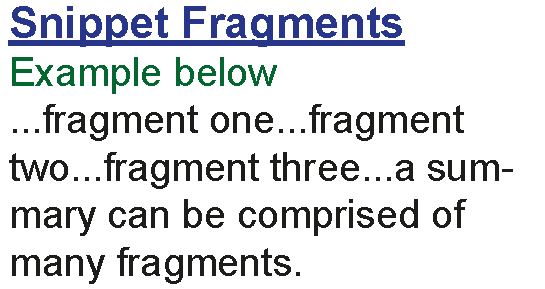
\includegraphics[width=1\textwidth]{figures/ch7-fragments.pdf}
    \end{center}
    \vspace*{-4mm}
    \label{fig:fragments}
\end{wrapfigure}

To decide the length and informativeness of the result summaries, we performed a preliminary analysis to determine the average length (in words) and informativeness (as calculated by the~\glsfirst{glos:kl}~\citep{kullback1951information} \todo{distance} to measure \emph{information gain}, or \emph{relative entropy}) of result summaries with the title, and a varying number of \emph{snippet fragments}\footnote{Figure~\ref{fig:serp_example} on page~\pageref{fig:serp_example} illustrates snippet fragments in the wider context of a~\gls{acr:serp}.} (from $0$ to $10$). The closer the entropy value is towards zero, the more information that is gained. Figure~\ref{fig:ig_plots} plots the number of words, the information gain, and the information gain attained per word.\footnote{These values were obtained by submitting over $300$ queries from a previous user study, conducted by~\cite{azzopardi2013query_cost}. These were conducted on similar topics, the same retrieval system and corpus used as the those used for this study.} It is clear from the plots shown in Figure~\ref{fig:ig_plots} that a higher level of information gain was present in longer snippets. However, as the length increased with each snippet fragment added, the informativeness per word also decreased. Consequently, we selected the four different interface conditions in the region where informativeness has the highest change, i.e. from zero to four. The conditions selected for this study were therefore:

\begin{figure}[t!]
    \centering
    \resizebox{1\hsize}{!}{
    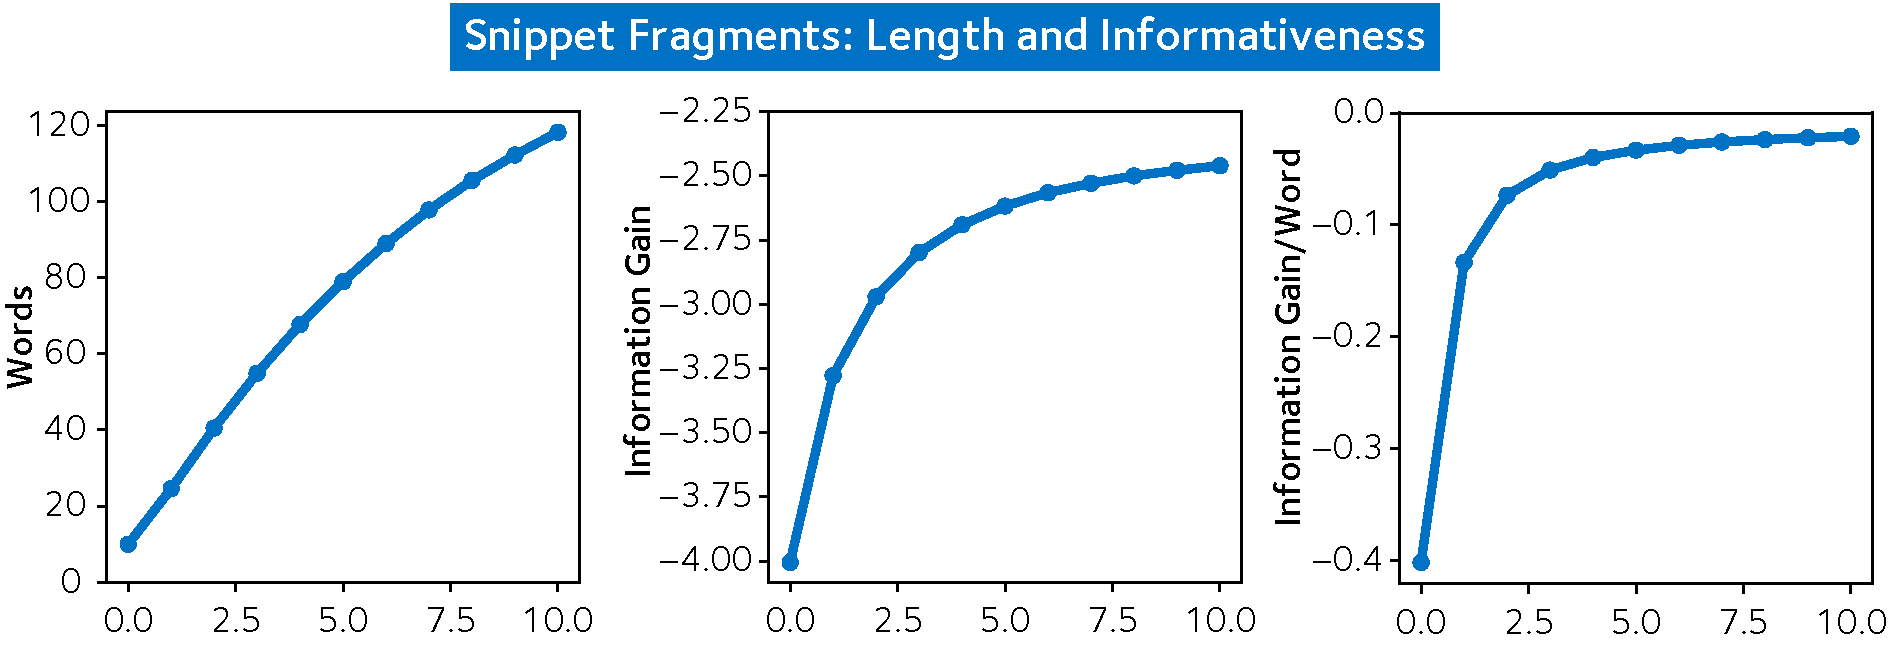
\includegraphics{figures/ch7-ig_plots.pdf}}
    \caption[Information gain plots]{Plots showing the length (in words), informativeness (in information gain, or \emph{IG}), and the information gain \emph{(IG)} per word for the title, plus 0 to 10 snippet fragments. The closer the value is to zero, the more information that is gained.}
    \label{fig:ig_plots}
\end{figure}

\begin{itemize}
    \item{\blueboxbold{T0}, where only the title for each result summary were presented;}
    \item{\blueboxbold{T1}, where for each result summary, a title and \emph{one} query-biased snippet fragment were presented;}
    \item{\blueboxbold{T2}, where a title and \emph{two} query-biased snippet fragments were presented; and}
    \item{\blueboxbold{T4}, where a title and \emph{four} query-biased snippet fragments were presented.}
\end{itemize}

For these interfaces, our independent variable was snippet informativeness, controlled by the length of the result summary snippets. Figure~\ref{fig:interface_snippets} provides a complete, rendered example of the different result summaries in each condition, using the same document.

From here, we carefully selected the order in which subjects were presented with each interface. For each of the four main topics discussed in Section~\ref{sec:methodology:collection:topics}, one of the four interfaces from \blueboxbold{T0}, \blueboxbold{T1}, \blueboxbold{T2} and \blueboxbold{T4} were assigned to a topic using a Latin-square rotation. For the practice topic, we used \blueboxbold{T2} -- a title and two snippet fragments -- the interface that represented the \emph{de facto} standard for presenting result summaries~\citep{hearst2009_search}.

\begin{figure}[t!]
    \centering
    \resizebox{1\hsize}{!}{
    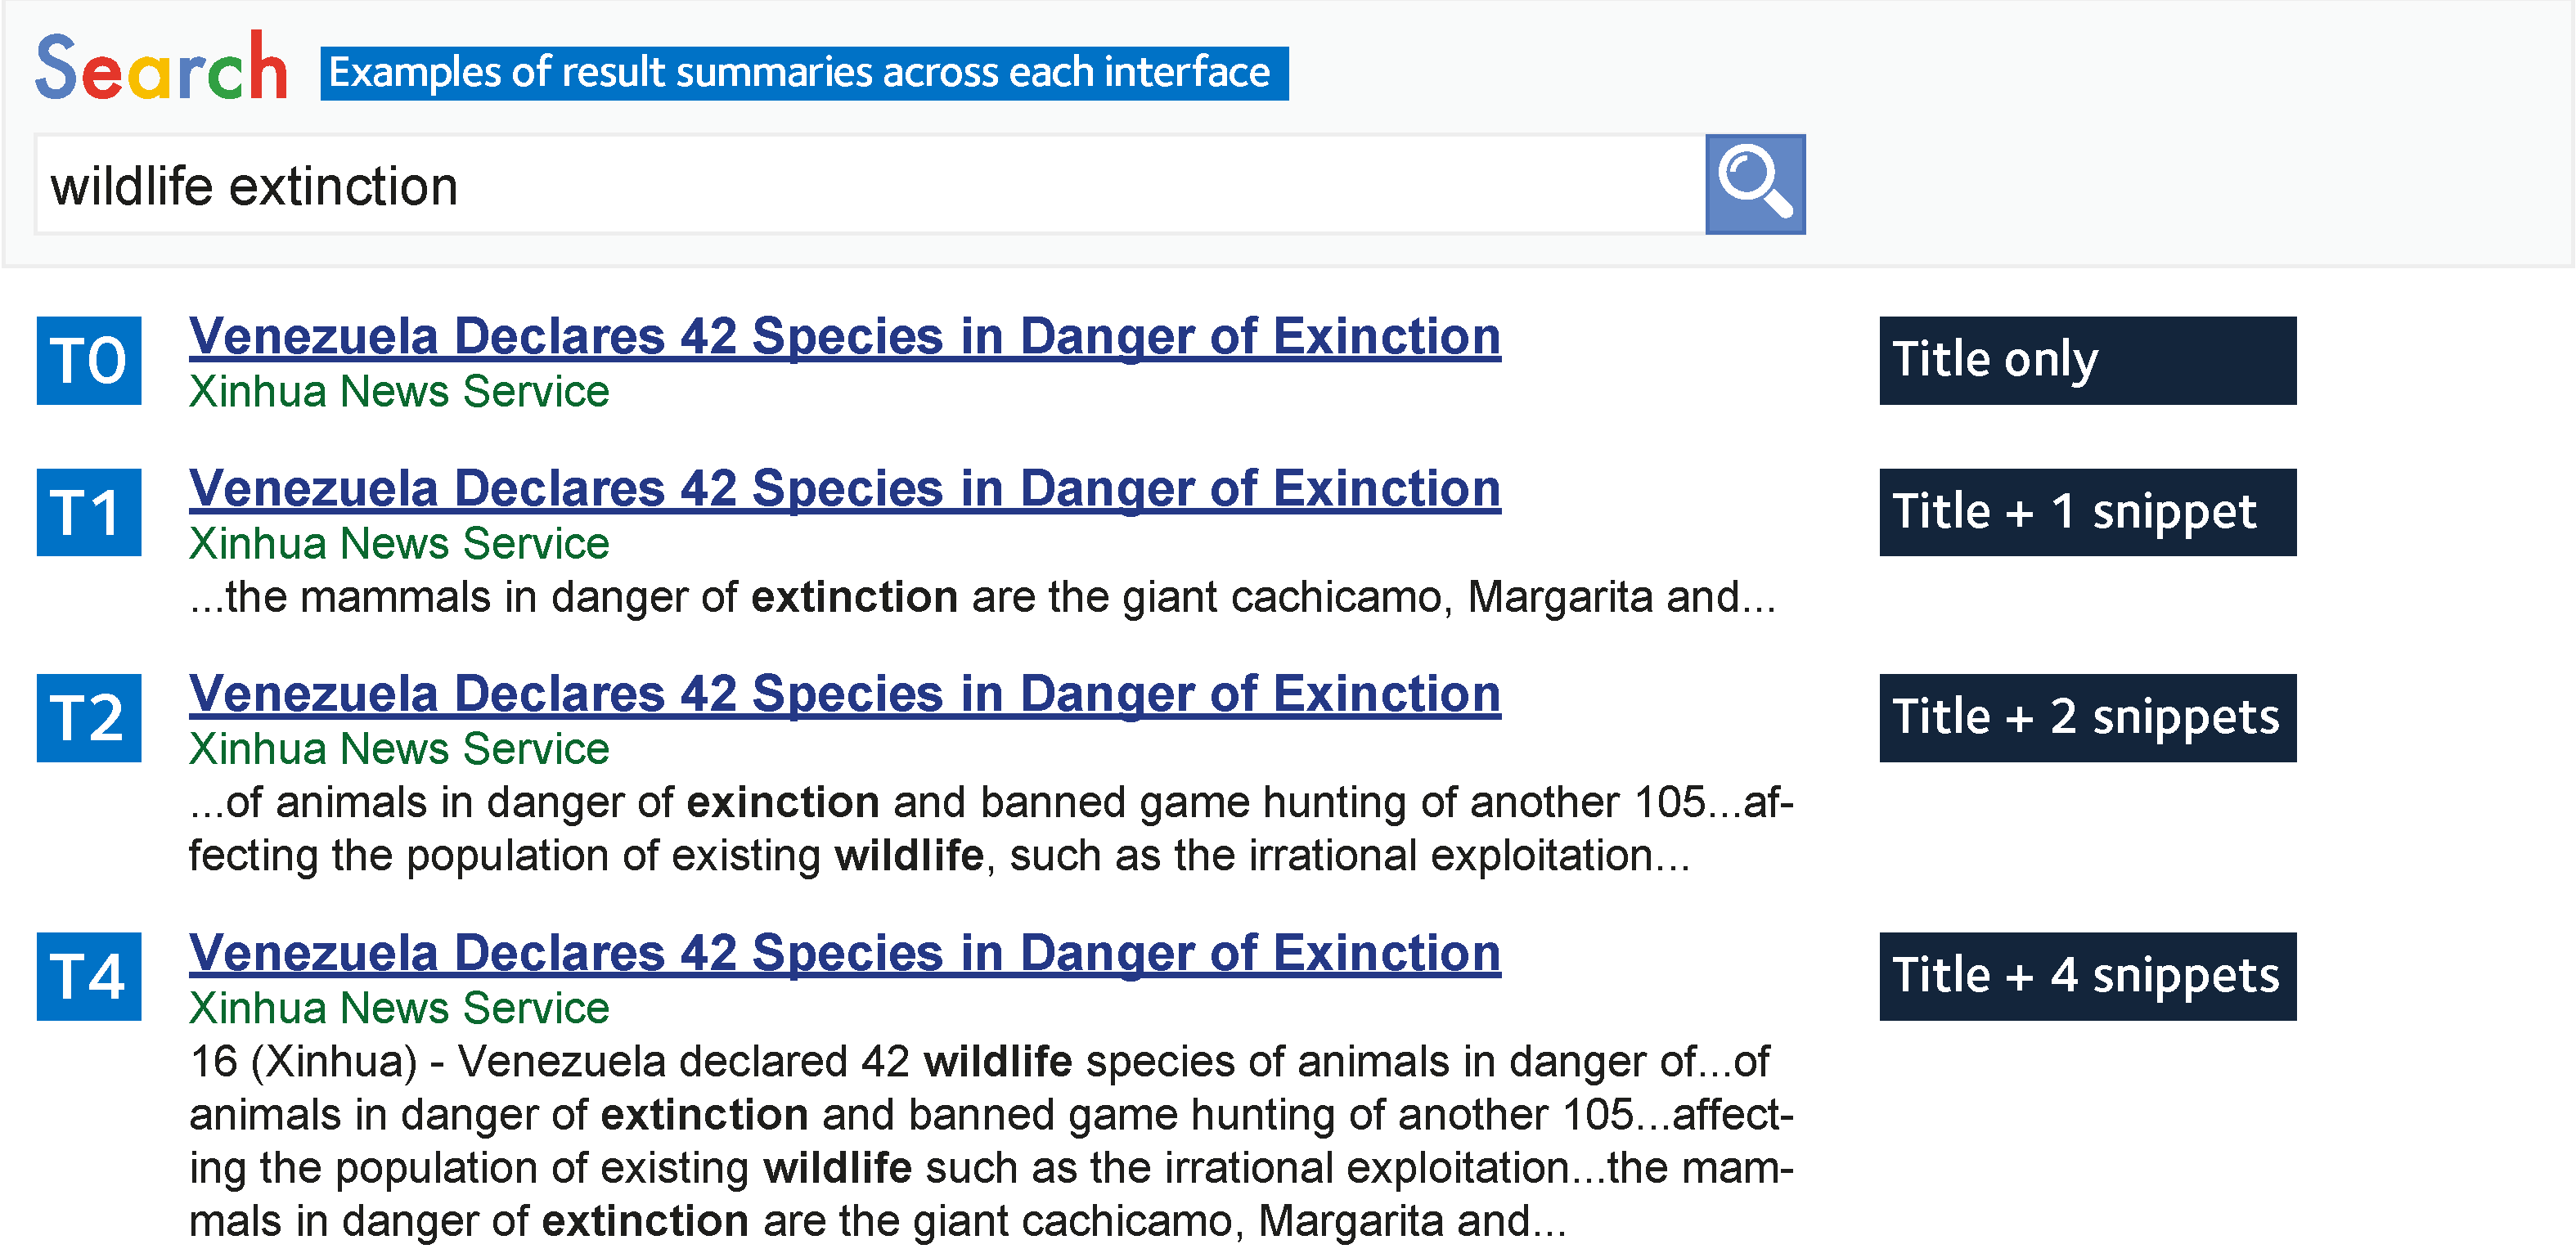
\includegraphics{figures/ch7-interface_snippets.pdf}}
    \caption[Examples of result summaries across experimental interfaces]{Examples of the result summaries generated by each of the four interfaces, \blueboxbold{T0}, \blueboxbold{T1}, \blueboxbold{T2} and \blueboxbold{T4} used in this study. The same document is used. Demonstrated by \searchlogo, each of the result summaries consists of: a title (in blue, underlined); none, one, or more snippet fragments (in black, with fragments separated by ellipses); and a newswire source (in green).}
    \label{fig:interface_snippets}
\end{figure}

\subsubsection{Snippet Generation}\label{sec:snippets:method:snippets}
For interfaces \blueboxbold{T2} to \blueboxbold{T4}, each result summary presented to the subjects required one or more snippet fragments from the corresponding document. As illustrated in the complete, rendered example in Figure~\ref{fig:interface_snippets}, each of the fragments generated were query-biased in nature~\citep{tombros1998query_biased}. Fragments were generated by splitting a given document into sentences (delimited by a full stop), and scoring each of the sentences according to BM25 (where $\beta=0.75$). Fragments were then extracted from the ordered series of sentences by identifying query terms within said sentences. Fragments were created by creating a window of $40$ characters from either side of the identified query term, as illustrated in the example figure below.

\begin{figure}[h]
    \centering
    \vspace{4mm}
    \resizebox{1\hsize}{!}{
    
\includegraphics{figures/ch7-fragment_example.pdf}}
    \label{fig:fragment_example}
    \vspace{-5mm}
\end{figure}

The ordered set of fragments were then joined together (one only for \blueboxbold{T1}, two for \blueboxbold{T2}, and four for \blueboxbold{T4}), separated by ellipses. These were combined together with the document's title and source newswire to form the complete result summary.

\subsubsection{Search Task}
As discussed previously in Section~\ref{sec:methodology:user:flow}, subjects were grounded by instructing them to imagine that they were newspaper reporters. As such, they were required to gather documents to write stories about each of the four topics they searched for. For this study, subjects were assigned ten minutes to each of the four search tasks, and were specifically instructed to find as many relevant documents as they could during this allotted time. As shown in Section~\ref{sec:methodology:user:interface}, subjects interacted with the standard search interface. Documents were \emph{saved} by subjects when they were considered to be relevant to the given~\gls{acr:trec} topic.

\subsubsection{Crowdsourced Subjects}\label{sec:snippets:method:subjects}
A total of $60$ subjects took part on the~\gls{acr:mturk} platform. However, seven subjects were omitted due to quality control constraints imposed on the study -- refer to Section~\ref{sec:methodology:user:crowdsourcing} for more information on the constrains imposed. This left $53$ subjects who satisfied the conditions of the experiment. In all, of the $53$ subjects who satisfied the criteria, $28$ were male, with the remaining $25$ female. The average age of the subjects was $33.8$ years ($min=22$; $max=48$; $stdev=7.0$). A total of $19$ subjects reported possessing a bachelor's degree or higher, and all expressing a high degree of search literacy, and conducted at least five searches for information online per week.

With a total of $53$ subjects considered in the results of this study, each searching over four topics, this meant a total of $212$ search sessions being logged and available for analysis. Finally, we report results over a reduced time period of six minutes ($360$ seconds). This decision was taken as not all of the $53$ subjects spent the full ten minutes searching, with these subjects skewing results. By reducing the time period that we considered, we ensured that we could extract meaningful data from the interaction logs, and guaranteed that subjects were interacting with the experimental system up until the cutoff point.

\subsubsection{Post-Task Surveys}\label{sec:snippets:method:posttask}
With the pre-task survey the same as that outlined in the general methodology (refer to Section~\ref{sec:methodology:extracting}), surveys for this study differed post-task and post-experiment. Here, we discuss the questions posed in each of the four post-task surveys.

A seven-point Likert scale was used for post-task surveys, similar to the pre-task surveys. Upon completion of each search task, the following statements were completed by each subject, selecting from \emph{strongly disagree} to \emph{strongly agree.}

\begin{itemize}
    \item{\blueboxbold{Clarity} The result summaries presented were clear and concise.}
    \item{\blueboxbold{Confidence} The result summaries presented increased my confidence in my decisions.}
    \item{\blueboxbold{Informativeness} The result summaries presented were informative to me.}
    \item{\blueboxbold{Relevance} The result summaries presented allowed me to judge the relevance of the associated document.}
    \item{\blueboxbold{Readability} The result summaries presented were readable.}
    \item{\blueboxbold{Size} The result summaries presented were of an appropriate size and length.}
\end{itemize}

These questions allowed us to obtain quantitative data alluding to how each subject perceived the search interface that they interacted with, and ascertain what they thought of the different result summary lengths.

\subsubsection{Post-Experiment Survey}\label{sec:snippets:method:postexperiment}
At the end of the experiment, subjects also completed a post-experiment survey. Five questions were posed, this time asking subjects to select which one of the four different interfaces best matched up with their opinion of the question asked.

\begin{itemize}
    \item{\blueboxbold{Most Informative?} Of the four interfaces, what one yielded the most informative result summaries?}
    \item{\blueboxbold{Least Helpful?} Of the four interfaces, which one provided the most unhelpful result summaries?}
    \item{\blueboxbold{Easiest?} Which of the four interfaces provided result summaries that were easiest to understand?}
    \item{\blueboxbold{Least Useful?} Of the four interfaces, which one provided the least useful result summaries?}
    \item{\blueboxbold{Most Preferred?} Of the four interfaces, what interface did you prefer using the most?}
\end{itemize}

These questions allowed us to determine which interface delivered the best impression overall across the five different questions asked.

\subsection{Results and Analysis}\label{chap:snippets:user:results}
From the four aspects we highlighted in Section~\ref{sec:methodology:extracting}, we report results from the study across four main sections, including analysis of:

\begin{itemize}
    \item{behavioural measures (interactions);}
    \item{time-based measures;}
    \item{performance measures; and}
    \item{user experience (surveys).}
\end{itemize}

Each measure was analysed over the four different search interfaces. To perform our analysis, \emph{Analysis of Variance (ANOVA) tests} were used using the interfaces as factors; main effects were examined with $\alpha = 0.05$. Bonferroni tests were used for post-hoc analysis.

\begin{table}[t!]
    \caption[Information gain across interfaces]{Characters, words and \emph{Information Gain (IG)} across each of the four interfaces trialled. An ANOVA test revealed \darkbluebox{significant differences}, with follow-up tests showing that each interface is significantly different to others. An IG value closer to zero denotes a higher level of IG. In the table below, \emph{IG/W.} denotes \emph{IG per word}.\vspace{-3mm}}
    \label{tbl:snippets_info_gain}
    \renewcommand{\arraystretch}{1.8}
    \begin{center}
    \begin{tabulary}{\textwidth}{L{3.75cm}@{\CS}D{2.6cm}@{\CS}D{2.6cm}@{\CS}D{2.6cm}@{\CS}D{2.6cm}}
    
    & \lbluecell\textbf{\emph{T0}} & \lbluecell\textbf{\emph{T1}} & \lbluecell\textbf{\emph{T2}} & \lbluecell\textbf{\emph{T4}}\\
    % OUTPUT FROM script
    
    \RS\lbluecell\textbf{Words} & \dbluecell 6.58$\pm$0.01 & \dbluecell 25.21$\pm$0.06 & \dbluecell44.29$\pm$0.10 & \dbluecell77.06$\pm$0.13 \\
    \RS\lbluecell\textbf{Characters} & \dbluecell37.37$\pm$0.05 & \dbluecell103.29$\pm$0.17 & \dbluecell168.36$\pm$0.23 & \dbluecell284.78$\pm$0.31 \\
    \RS\lbluecell\textbf{IG} & \dbluecell-6.35$\pm$0.01 & \dbluecell-3.59$\pm$0.00 & \dbluecell-3.00$\pm$0.00 & \dbluecell-2.67$\pm$0.00 \\
    \RS\lbluecell\textbf{IG/Word} & \dbluecell-1.17$\pm$0.00 & \dbluecell-0.18$\pm$0.00 & \dbluecell-0.08$\pm$0.00 & \dbluecell-0.04$\pm$0.00 \\
    
\end{tabulary}
\end{center}
\end{table}

To check whether the interfaces were sufficiently different with respect to snippet length and information gain, we performed an analysis of the result summaries that were presented to the subjects. Table~\ref{tbl:snippets_info_gain} summarises, over each interface, the number of words and characters that result summaries contained on average. As expected, the table shows an increasing trend of words and characters as the number of snippet fragments were increased. Information gain (or relative entropy), as previously discussed, was calculated using~\gls{glos:kl}~\citep{kullback1951information}.

Statistical testing showed that the differences between snippet length ($F(3,208 = 1.2x10^5, p<0.001)$) and information gain ($F(3,208) = 2.6x10^5, p<0.001)$) were significant. Follow up tests revealed that this was the case over all four interfaces, indicating that our conditions were indeed different on these dimensions.

These findings provide some justification for our choices of the number of snippet fragments used with each interface. A diminishing increase in information gain after four snippet fragments suggested that there would not have been much point generating result summaries that were any longer.

\begin{table}[t!]
    \caption[Behaviour and performance over experimental interfaces]{Various measures reported over each of the four experimental interfaces, \blueboxbold{T0}, \blueboxbold{T1}, \blueboxbold{T2} and \blueboxbold{T4}. Included are interaction and time-based measures (behavioural), as well as performance-based measures. No significant differences were observed, bar for the time per result summary, as \darkbluebox{highlighted}. Refer to Section~\ref{chap:snippets:user:results:time} for details.}
    \label{tbl:snippets_intperftime}
    \renewcommand{\arraystretch}{1.8}
    \begin{center}
    \begin{tabulary}{\textwidth}{L{0.4cm}@{\CS}L{3.2cm}@{\CS}D{2.5cm}@{\CS}D{2.5cm}@{\CS}D{2.5cm}@{\CS}D{2.5cm}@{\CS}}

        & & \lbluecell \textbf{T0} & \lbluecell \textbf{T1} & \lbluecell \textbf{T2} & \lbluecell \textbf{T4} \\

        \RS \multirow{4}{*}{\rotatebox{90}{\hspace*{-5mm}\textbf{Interactions}}} & \lbluecell\textbf{\#Queries} & \cell \small{3.72$\pm$0.34} & \cell \small{3.19$\pm$0.35} & \cell \small{3.30$\pm$0.35} & \cell \small{3.28$\pm$0.31}\\
        \RS & \lbluecell\textbf{\#\glsplural{acr:serp}/Query} & \cell \small{2.87$\pm$0.29} & \cell \small{2.69$\pm$0.23} & \cell \small{2.43$\pm$0.13} & \cell \small{2.40$\pm$0.20}\\
        \RS & \lbluecell\textbf{\#Docs./Query} & \cell \small{4.23$\pm$0.55} & \cell \small{4.83$\pm$0.54} & \cell \small{5.14$\pm$0.66} & \cell \small{4.76$\pm$0.62}\\
        \RS & \lbluecell\textbf{Depth/Query} & \cell \small{15.44$\pm$1.81} & \cell \small{17.00$\pm$2.21} & \cell \small{14.37$\pm$1.39} & \cell \small{13.53$\pm$1.95}\\
        
        \RS\RS\RS \multirow{4}{*}{\rotatebox{90}{\hspace*{-5mm}\textbf{Performance}}} & \lbluecell\textbf{P@10} & \cell \small{0.25$\pm$0.02} & \cell \small{0.23$\pm$0.02} & \cell \small{0.27$\pm$0.02} & \cell \small{0.25$\pm$0.03}\\
        \RS & \lbluecell\textbf{\#Saved} & \cell \small{6.68$\pm$0.66} & \cell \small{7.00$\pm$0.63} & \cell \small{6.49$\pm$0.58} & \cell \small{7.60$\pm$0.79}\\
        \RS & \lbluecell\textbf{\#\gls{acr:trec} Saved} & \cell \small{2.58$\pm$0.34} & \cell \small{2.28$\pm$0.25} & \cell \small{2.47$\pm$0.28} & \cell \small{2.66$\pm$0.32}\\
        \RS & \lbluecell\textbf{\#\gls{acr:trec} Non.} & \cell \small{1.85$\pm$0.32} & \cell \small{2.08$\pm$0.29} & \cell \small{1.98$\pm$0.24} & \cell \small{1.68$\pm$0.32}\\
        
        \RS\RS\RS \multirow{3}{*}{\rotatebox{90}{\hspace*{-5mm}\textbf{Times}}} & \lbluecell\textbf{Per Query} & \cell \small{8.29$\pm$0.57} & \cell \small{7.99$\pm$0.57} & \cell \small{9.42$\pm$0.79} & \cell \small{8.12$\pm$0.48}\\
        \RS & \lbluecell\textbf{Per Document} & \cell \small{17.32$\pm$2.12} & \cell \small{22.82$\pm$6.03} & \cell \small{17.19$\pm$1.86} & \cell \small{18.99$\pm$2.13}\\
        \RS & \lbluecell\textbf{Per Summary} & \dbluecell \small{1.63$\pm$0.13} & \cell \small{2.21$\pm$0.21} & \cell \small{2.35$\pm$0.23} & \dbluecell \small{2.60$\pm$0.27}\\
        
    \end{tabulary}
    \end{center}
\end{table}

\subsubsection{Interaction Measures}
Across the four experimental interfaces trialled, Table~\ref{tbl:snippets_intperftime} presents the mean ($\pm$ standard deviations) of:

\begin{itemize}
    \item{the number of queries issued \genericblack{(\#Queries)};}
    \item{the number of~\gls{acr:serp} viewed per query \genericblack{(\#\glsplural{acr:serp}/Query)};}
    \item{the number of documents viewed per query \genericblack{(\#Docs./Query)}; and}
    \item{the mean click depth -- or stopping depth \genericblack{(Depth/Query)}.}
\end{itemize}

These are all presented within the \genericblack{Interactions}~grouping. Across the four experimental interfaces of \blueboxbold{T0}, \blueboxbold{T1}, \blueboxbold{T2} and \blueboxbold{T4}, there were no significant differences reported between any of these measures. The number of queries issued follows a slight downward trend as the length of the result summaries (dictated by the interface conditions) increased ($3.72 \pm 0.34$ for \blueboxbold{T0}, to $3.28\pm0.31$ for \blueboxbold{T4}). This was also true for the number of~\glsplural{acr:serp} examined, and the number of documents examined per query. The depth to which subjects went to per query however follows a downward trend. As the length of each result summary increased, subjects were likely to go to shallower depths per query when examining result summaries ($24.47\pm2.96$ for \blueboxbold{T0}, to $19.4\pm20.04$ for \blueboxbold{T4}).

\begin{table}[t!]
    \caption[Interaction probabilities]{A summary of the various interaction probabilities over each of the four experimental interfaces examined. Note the increasing trends for each probability from \blueboxbold{T0} $\rightarrow$ \blueboxbold{T4}. Section~\ref{sec:method:simulation:grounding:judgements} on page~\pageref{sec:method:simulation:grounding:judgements} provides an explanation of the various probabilities listed here.}
    \label{tbl:snippets_probabilities}
    \renewcommand{\arraystretch}{1.8}
    \begin{center}
    \begin{tabulary}{\textwidth}{L{0.4cm}@{\CS}L{3.2cm}@{\CS}D{2.5cm}@{\CS}D{2.5cm}@{\CS}D{2.5cm}@{\CS}D{2.5cm}@{\CS}}

        \RS & & \lbluecell \textbf{T0} & \lbluecell \textbf{T1} & \lbluecell \textbf{T2} & \lbluecell \textbf{T4} \\

        \RS \multirow{3}{*}{\rotatebox{90}{\hspace*{-5mm}\textbf{Click}}} & \lbluecell\textbf{P(C)} & \cell \small{0.20$\pm$0.02} & \cell \small{0.25$\pm$0.02} & \cell \small{0.26$\pm$0.03} & \cell \small{0.28$\pm$0.03}\\
        \RS & \lbluecell\textbf{P(C|R)} & \cell \small{0.28$\pm$0.03} & \cell \small{0.34$\pm$0.03} & \cell \small{0.35$\pm$0.03} & \cell \small{0.40$\pm$0.04}\\
        \RS & \lbluecell\textbf{P(C|N)} & \cell \small{0.18$\pm$0.02} & \cell \small{0.23$\pm$0.02} & \cell \small{0.25$\pm$0.03} & \cell \small{0.24$\pm$0.03}\\
        
        \RS\RS\RS \multirow{3}{*}{\rotatebox{90}{\hspace*{-5mm}\textbf{Save}}} & \lbluecell\textbf{P(S)} & \cell \small{0.61$\pm$0.04} & \cell \small{0.68$\pm$0.04} & \cell \small{0.65$\pm$0.03} & \cell \small{0.71$\pm$0.03}\\
        \RS & \lbluecell\textbf{P(S|R)} & \cell \small{0.66$\pm$0.06} & \cell \small{0.69$\pm$0.05} & \cell \small{0.67$\pm$0.05} & \cell \small{0.66$\pm$0.05}\\
        \RS & \lbluecell\textbf{P(S|N)} & \cell \small{0.55$\pm$0.04} & \cell \small{0.65$\pm$0.04} & \cell \small{0.58$\pm$0.04} & \cell \small{0.67$\pm$0.04}\\
        
    \end{tabulary}
    \end{center}
\end{table}

Interaction probabilities all showed an increasing trend as result summary length increased over the four experimental interfaces, as shown in Table~\ref{tbl:snippets_probabilities}. Explanations for what each of the different probabilities represent can be found in Section~\ref{sec:method:simulation:grounding:judgements} on page~\pageref{sec:method:simulation:grounding:judgements}. Although no significant differences were observed over the four interfaces and the different probabilities examined, trends across all probabilities show an increase as result summary length increased. An increase of both the probability of clicking result summaries on the~\gls{acr:serp} ($P(C)$) and saving the associated documents ($P(S)$) as relevant were observed. When these probabilities are examined in more detail by separating the result summaries clicked and documents saved by their~\gls{acr:trec} relevancy, we see increasing trends for clicking and saving -- both for~\gls{acr:trec} relevant ($P(C|R)$ and $P(S|R)$ for clicking and saving, respectively), and~\gls{acr:trec} non-relevant documents ($P(C|N)$ and $P(M|N)$). This interesting finding shows that an increase in result summary length does not necessarily improve a subject's accuracy, but simply the likelihood that they will consider documents to be relevant.


\subsubsection{Time-Based Measures}\label{chap:snippets:user:results:time}
Table~\ref{tbl:snippets_intperftime} also presents three time-based measures (within the \genericblack{Times}~grouping) that were observed across the four experimental interfaces. We show:

\begin{itemize}
    \item{the mean time spent by subjects issuing queries \genericblack{(Per Query)};}
    \item{the mean time spent by subjects examining individual documents \genericblack{(Per Document)}; and}
    \item{the mean time spent examining individual result summaries \genericblack{(Per Summary)}.}
\end{itemize}

\begin{figure}[t!]
    \centering
    \resizebox{1\hsize}{!}{
    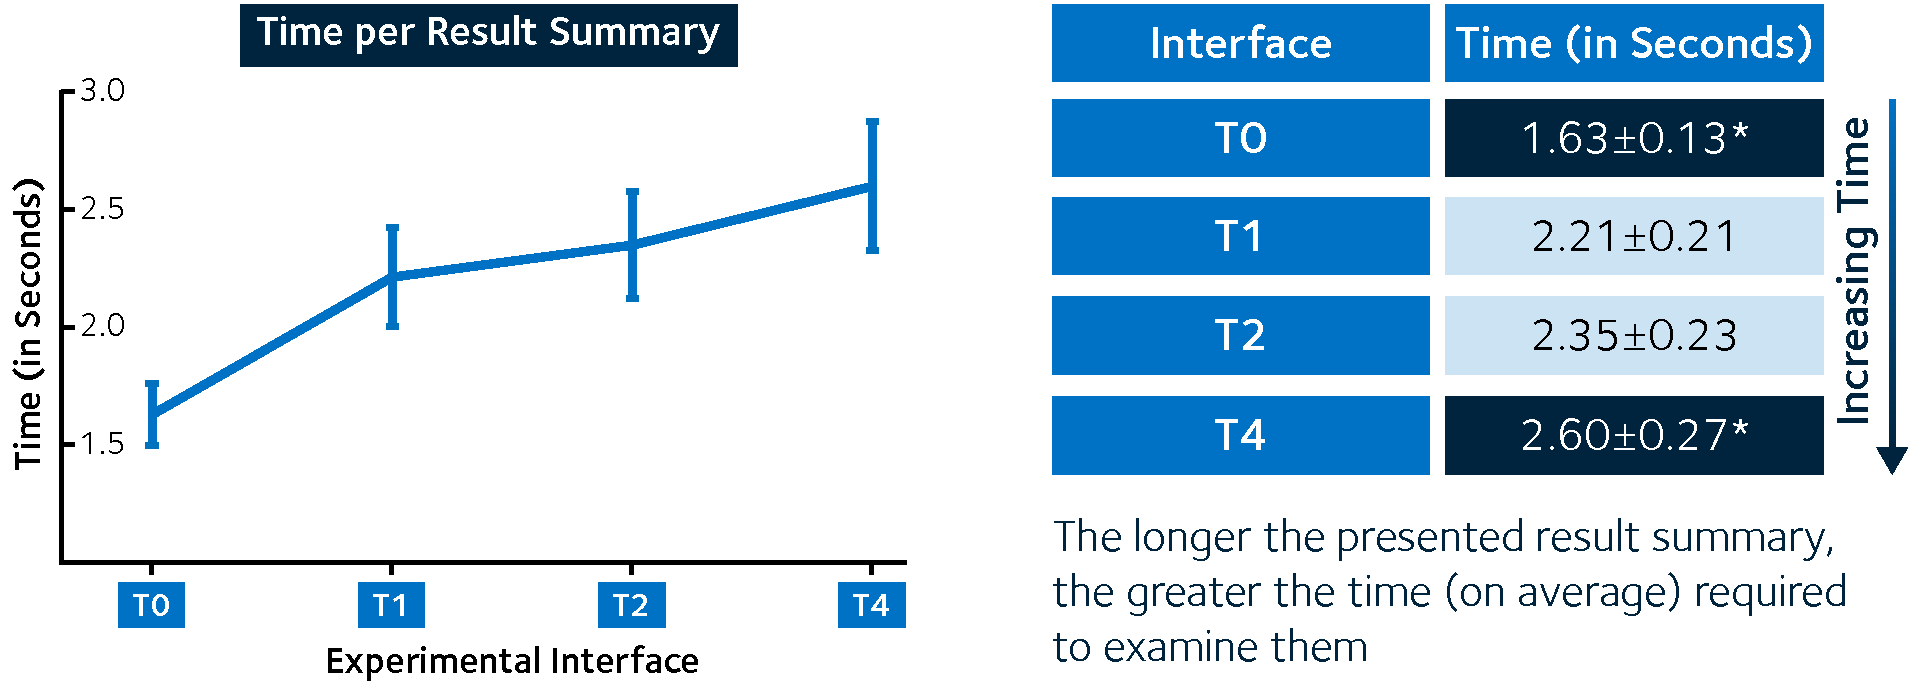
\includegraphics{figures/ch7-time_snippet.pdf}}
    \caption[Time per result summary]{Plot and table illustrating the mean time spent examining result summaries across each of the four experimental interfaces trialled. Note the increasing mean examination time as the result summary length increases, from \blueboxbold{T0} $\rightarrow$ \blueboxbold{T4}. Error bars denote the standard deviation.}
    \label{fig:time_snippet}
\end{figure}

No significant differences were found between the time spent per query, and the time spent examining individual documents. However, a significant difference did exist for the time spent per result summary, as can be seen from the table. A clear upward trend in the time spent examining result summaries can be seen in Figure~\ref{fig:time_snippet} as result summaries progressively got longer, from $1.63\pm0.13$ for \blueboxbold{T0} to $2.6\pm0.27$ for \blueboxbold{T4}, which was significantly different ($F(3,208) = 3.6, p=0.014$). The follow-up Bonferroni test showed that the significant difference did exist between interfaces \blueboxbold{T0} and \blueboxbold{T4}. This finding suggests that as result summary length increases, the amount of time spent examining individual result summaries also increases, presenting us with an intuitive result. This also complies with trends observed regarding examination depths. When the length of result summaries increased, subjects were likely to examine result summaries to shallower depths.

\subsubsection{Performance}
Also included within Table~\ref{tbl:snippets_intperftime} are our reported performance measures, this time shown under the \genericblack{Performance}~grouping. Again, these are reported over each of the four experimental interfaces trialled. We report the mean performance of:

\begin{itemize}
    \item{the issued queries, with the \genericblack{P@10} score;}
    \item{the number of documents that were saved by subjects \genericblack{(\#Saved);}}
    \item{the interactive precision, or the number of saved documents that were~\gls{acr:trec} relevant \genericblack{(\#\gls{acr:trec} Saved);} and also}
    \item{the number of saved documents that were not~\gls{acr:trec} relevant \genericblack{(\#\gls{acr:trec} Non.).}}
\end{itemize}

Like the interaction measures examined previously, no significant differences were observed over the four experimental interfaces examined. The performance of queries issued by subjects was very similar across all interfaces ($P@10 \approx 0.25$), along with the number of documents identified by subjects as relevant ($6.49\pm0.58$) for \blueboxbold{T2} to $7.6\pm0.79$ for \blueboxbold{T4}, and the interactive precision ($2.28\pm0.25$ for \blueboxbold{T1} to $2.66\pm0.32$ for \blueboxbold{T4}). Considering the number of saved,~\gls{acr:trec} non-relevant documents, where subjects on averaged saved two such documents. However, there again no significant differences between the four interfaces.

\subsubsection{User Experience}\label{chap:snippets:user:results:ux}
In this section, we analyse the results of the post-task and post-experiment surveys that subjects completed. Examining the results from these surveys allow us to capture the subject's perceived experiences of using the experimental system across all four interfaces trialled.

\begin{table}[t!]
    \caption[Post-task survey results]{Summary table of the recorded observations for the post-task surveys, indicating the preferences of subjects over the six criteria and four experimental interfaces. Across all criteria, \blueboxbold{T0} was \darkbluebox{significantly different} from the other three interfaces. Using the seven-point Likert scale, results are shown from 1 (strongly disagree) to 7 (strongly agree).}
    \label{tbl:snippets_posttask}
    \renewcommand{\arraystretch}{1.8}
    \begin{center}
    \begin{tabulary}{\textwidth}{L{4.15cm}@{\CS}D{2.5cm}@{\CS}D{2.5cm}@{\CS}D{2.5cm}@{\CS}D{2.5cm}@{\CS}}

        \RS & \lbluecell \textbf{T0} & \lbluecell \textbf{T1} & \lbluecell \textbf{T2} & \lbluecell \textbf{T4} \\

        \RS \lbluecell\textbf{Clarity} & \dbluecell \small{4.16$\pm$0.27*} & \cell \small{5.00$\pm$0.21} & \cell \small{5.06$\pm$0.24} & \cell \small{5.40$\pm$0.20}\\
        \RS \lbluecell\textbf{Confidence} & \dbluecell \small{3.71$\pm$0.26*} & \cell \small{4.66$\pm$0.26} & \cell \small{4.75$\pm$0.24} & \cell \small{5.06$\pm$0.25}\\
        \RS \lbluecell\textbf{Informativeness} & \dbluecell \small{4.20$\pm$0.30*} & \cell \small{5.38$\pm$0.24} & \cell \small{5.27$\pm$0.24} & \cell \small{5.62$\pm$0.20}\\
        \RS \lbluecell\textbf{Relevance} & \dbluecell \small{3.84$\pm$0.28*} & \cell \small{4.89$\pm$0.25} & \cell \small{5.08$\pm$0.24} & \cell \small{5.36$\pm$0.20}\\
        \RS \lbluecell\textbf{Readability} & \dbluecell \small{5.18$\pm$0.31*} & \cell \small{6.32$\pm$0.17} & \cell \small{6.46$\pm$0.14} & \cell \small{6.36$\pm$0.14}\\
        \RS \lbluecell\textbf{Size} & \dbluecell \small{4.00$\pm$0.31*} & \cell \small{4.94$\pm$0.25} & \cell \small{5.21$\pm$0.22} & \cell \small{5.36$\pm$0.19}\\
        
    \end{tabulary}
    \end{center}
\end{table}

\blueboxheader{Post-Task Surveys}
Table~\ref{tbl:snippets_posttask} presents the mean set of results (and their standard deviations) from subjects across the four interfaces trialled. As previously discussed, these questions were answered upon the completion of each search task. The survey questions are detailed in Section~\ref{sec:snippets:method:posttask}. Using a seven-point Likert scale for their responses (with $1$ denoting a strong disagreement, and $7$ denoting a strong agreement), significant differences were found in all question responses, as shown below.

\begin{itemize}
    \item{\blueboxbold{Clarity} $F(3,208)=5.22, p=0.001$}
    \item{\blueboxbold{Confidence} $F(3,208)=5.2, p=0.001$}
    \item{\blueboxbold{Informativeness} $F(3,208)=5.22, p=0.001$}
    \item{\blueboxbold{Relevance} $F(3,208)=6.44, p<0.001$}
    \item{\blueboxbold{Readability} $F(3,208)=9.25, p<0.001$}
    \item{\blueboxbold{Size} $F(3,208)=7.28, p<0.001$}
\end{itemize}

Follow-up Bonferroni tests however shows that the significant difference existed only between \blueboxbold{T0} and the remaining three interfaces, \blueboxbold{T1}, \blueboxbold{T2} and \blueboxbold{T4}. A series of discernible trends can be observed throughout the responses, with subjects regarding longer result summaries as more concise, and a possessing a higher degree of clarity ($4.16\pm0.27$ for \blueboxbold{T0} to $5.4\pm0.2$ for \blueboxbold{T4}). This perceived clarity also made subjects feel more confidence that the longer result summaries helped them make better decisions as to whether they were relevant to the given topic. Interaction results presented above however differ from this (as shown in Table~\ref{tbl:snippets_probabilities}), where the overall probability of saving documents increased, regardless of the document/topic relevancy judgement. Other notable trends observed from the results included an increase in how informative subjects perceived results to be -- again, with longer result summaries proving to be more informative. Subjects also reported a general increase in satisfaction of the length of the presented result summaries. However, as mentioned, no significant difference existed between the three interfaces in which snippets were generated as part of the result summaries (i.e. \blueboxbold{T1}, \blueboxbold{T2} and \blueboxbold{T4}).

\blueboxheader{Post-Experiment Survey}
As detailed previously in Section~\ref{sec:snippets:method:postexperiment}, subjects completed a post-experiment exit survey. Responses from the subjects are presented in Table~\ref{tbl:snippets_postexp}. From the results, subjects found result summaries of longer lengths (i.e. those generated by interfaces \blueboxbold{T2} and \blueboxbold{T4}) to be the most informative, and those generated by \blueboxbold{T0} -- without any snippet(s) -- to be the least helpful and useful. The longer result summaries were also consistently favoured by subjects who preferred them over the result summaries generated by interfaces \blueboxbold{T0} and \blueboxbold{T1}. Subjects also found the result summaries of longer length easier to use to satisfy the given information need.

From the results, it is therefore clear that a majority of subjects preferred longer result summaries to be presented on~\glsplural{acr:serp}, generated by interfaces \blueboxbold{T2} and \blueboxbold{T4}. This is illustrated in Table~\ref{tbl:snippets_postexp} by the \darkbluebox{highlighting} of the key results.

\begin{table}[t!]
    \caption[Post-experiment survey results]{Raw results of responses from the post-experiment exit survey completed by each subject. More information on the survey can be found in Section~\ref{sec:snippets:method:postexperiment}, with results discussed in Section~\ref{chap:snippets:user:results:ux}.}
    \label{tbl:snippets_postexp}
    \renewcommand{\arraystretch}{1.8}
    \begin{center}
    \begin{tabulary}{\textwidth}{L{4.15cm}@{\CS}D{2.5cm}@{\CS}D{2.5cm}@{\CS}D{2.5cm}@{\CS}D{2.5cm}@{\CS}}

        \RS & \lbluecell \textbf{T0} & \lbluecell \textbf{T1} & \lbluecell \textbf{T2} & \lbluecell \textbf{T4} \\

        \RS \lbluecell\textbf{Most Informative} & \cell \small{1} & \cell \small{4} & \dbluecell \small{20} & \dbluecell \small{29}\\
        \RS \lbluecell\textbf{Least Helpful} & \dbluecell \small{46} & \cell \small{5} & \cell \small{1} & \cell \small{2}\\
        \RS \lbluecell\textbf{Easiest} & \cell \small{4} & \cell \small{4} & \dbluecell \small{24} & \dbluecell \small{22}\\
        \RS \lbluecell\textbf{Least Useful} & \dbluecell \small{49} & \cell \small{4} & \cell \small{0} & \cell \small{1}\\
        \RS \lbluecell\textbf{Most Preferred} & \cell \small{3} & \cell \small{5} & \dbluecell \small{20} & \dbluecell \small{26}\\
        
    \end{tabulary}
    \end{center}
\end{table}

\subsection{Discussion and User Study Conclusions}
This user study investigated the influence of result summary length on search behaviour and performance. Using Kullback-Leibler distance~\citep{kullback1951information} as a measure of information gain, we examined result summaries of different lengths, selected a series of result summary lengths (comprised of snippet fragments) where there was a significant difference in information gain between them, which yielded the configurations for our four experimental conditions, \blueboxbold{T0}, \blueboxbold{T1}, \blueboxbold{T2} and \blueboxbold{T4}. A crowdsourced, within-subjects user study was performed comprising of 53 subjects, each of whom undertook four search tasks, using each of the four experimental interfaces.

This work was focused around addressing the two key research questions, which explored \darkblueboxbold{RQ1} how the length of a result summary affected search behaviour and user experience; and \darkblueboxbold{RQ2} whether the length of result summaries affected the decision making ability and accuracy of the subjects.

Addressing \darkblueboxbold{RQ1} first in terms of search behaviour, there was admittedly little difference -- but we did observe the following trends. As result summary length increased, subjects:

\begin{itemize}
    \item{issued fewer queries and examined fewer pages; \emph{but importantly}}
    \item{\emph{clicked more documents.}}
\end{itemize}

These findings demonstrate that subjects would spend more of their time assessing documents at deeper ranks. Our results also show that in terms of experience, subjects broadly preferred longer result summaries. The subjects felt that longer summaries were more clear, informative, and readable. In addition to this, the longer result summaries also gave subjects more confidence in their relevance decisions.

With respect to \blueboxbold{RQ2}, we again observed little difference in subjects' decision making abilities and accuracy between the four experimental interfaces. While subjects perceived longer result summaries to help them infer relevance more accurately, our empirical evidence suggests otherwise. In fact, it would appear that longer result summaries were more attractive, increasing the information scent of the~\gls{acr:serp}. This may account for the increase in clicks on the early results, without the benefits, however: accuracy of our subjects did not improve with longer result summaries, nor did they find more relevant documents. Increased confidence in the result summaries (from interfaces \blueboxbold{T0} $\rightarrow$ \blueboxbold{T4}) may have led to a more relaxed approach at saving content as relevant -- as can be seen by increasing click and mark probabilities for both relevant and non-relevant content. It is also possible that the \emph{paradox of choice}~\citep{oulasvirta2009serp_size} could play a role in shaping a searcher's preferences. For example, in the interface with the longest result summaries, \blueboxbold{T4}, subjects viewed fewer results/choices than on other conditions. This may have contributed to their feelings of greater satisfaction and increased confidence in their decisions.

These novel findings provide new insights into how searchers interact with result summaries in terms of their experiences and search behaviours. Previous work had only focused upon task completion times and accuracy of the first result while not considering their experiences~\citep{cutrell2007eye_tracking, kaisser2008improving}. Our findings show that longer result summaries, while containing a greater amount of information content, are not necessarily better in terms of decision making -- although subjects perceived this to be the case. We also show a positive relationship between the length and informativeness of result summaries and their attractiveness (clickthrough rates). These results show that the experiences and perceptions of searchers -- and the actual performance of those searchers -- is different, and when designing interfaces, this needs to be taken into account.

\section{Simulated Analysis}\label{sec:snippets:simulations}
We now move from the user study reported above to a simulated analysis, examining closely how stopping behaviour varies when searchers are subjected to result summaries of varying length. In particular, this section provides results and discussion of an extensive set of simulations, examining how the twelve different result summary level stopping strategies (defined in Chapter~\ref{chap:strategies}):

\begin{itemize}
    \item{\darkblueboxbold{HL-RQ3a} perform; and}
    \item{\darkblueboxbold{HL-RQ3b} how closely they approximate actual searcher stopping behaviour.}
\end{itemize}

For both research questions, these are addressed under the context of what happens to performance and approximations when result summary lengths are varied. In the remainder of this section, we provide methodology details specific to this study (Section~\ref{sec:snippets:simulations:method}), before providing the results of the simulations (Section~\ref{sec:snippets:simulations:results}).

\subsection{Methodology}\label{sec:snippets:simulations:method}
This small methodology section outlines the details specific to this set of simulations. One can assume that any components not discussed here were instantiated as presented in the general simulation methodology, as discussed in Section~\ref{sec:method:simulation} on page~\pageref{sec:method:simulation}.

As we wish to examine how stopping behaviour varies when searchers are exposed to interfaces yielding result summaries of different lengths, we utilised all four of the experimental interfaces discussed previously in this simulation study. Below, we discuss the interfaces used (Section~\ref{sec:snippets:simulations:method:interfaces}), before outlining the interaction costs and probabilities extracted for each interface (Section~\ref{sec:method:simulation:grounding:costs}).

\subsubsection{Experimental System and Interfaces}\label{sec:snippets:simulations:method:interfaces}
The experimental system used for these simulations was largely the same as outlined in Section~\ref{sec:method:simulation} on page~\pageref{sec:method:simulation} -- save for the incorporation of the snippet generation components as outlined previously in Section~\ref{sec:snippets:method:snippets} within the \simiir~framework.

By incorporating this component, this allowed us to run simulations that presented to simulated searchers four different interfaces, namely \blueboxbold{T0}, \blueboxbold{T1}, \blueboxbold{T2}, and \blueboxbold{T4}. This allowed us to mirror as closely as possible -- given the experimental setup -- the interfaces that the real-world searchers were subjected to in the associated user study.

\subsubsection{Interaction Costs and Probabilities}\label{sec:snippets:simulations:method:costs}
We then took the interaction log data from the associated user study. For each of the four experimental interfaces trialled in the user study, we could then, following the methodology outlined in Sections~\ref{sec:method:simulation:grounding:judgements} and~\ref{sec:method:simulation:grounding:costs}, extract the different interaction probabilities and costs to ground our simulations.

\begin{table}[t!]
    \caption[Simulation interaction probabilities and costs (result summaries)]{Summary table of the different interaction costs (in seconds) and probabilities, with \emph{P(C)} denoting the probability of a click, and \emph{P(S)} denoting the probability of saving a document (considering it relevant). Refer to Sections~\ref{sec:method:simulation:grounding:costs} and~\ref{sec:method:simulation:grounding:judgements} respectively for further information on how the costs and probabilities were derived. All data in this table is attained from interaction data extracted from the user study reported in Section~\ref{chap:snippets:user}.}
    \label{tbl:snippets_simulation_probcosts}
    \renewcommand{\arraystretch}{1.8}
    \begin{center}
    \begin{tabulary}{\textwidth}{L{0.4cm}@{\CS}L{3.2cm}@{\CS}D{2.5cm}@{\CS}D{2.5cm}@{\CS}D{2.5cm}@{\CS}D{2.5cm}@{\CS}}

        \RS & & \lbluecell \textbf{T0} & \lbluecell \textbf{T1} & \lbluecell \textbf{T2} & \lbluecell \textbf{T4} \\

        \RS \multirow{2}{*}{\rotatebox{90}{\hspace*{-2mm}\textbf{P(C)}}} & \lbluecell\textbf{P(C|R)} & \cell \small{0.28} & \cell \small{0.34} & \cell \small{0.35} & \cell \small{0.40}\\
        \RS & \lbluecell\textbf{P(C|N)} & \cell \small{0.18} & \cell \small{0.23} & \cell \small{0.25} & \cell \small{0.24}\\
        
        \RS\RS\RS \multirow{2}{*}{\rotatebox{90}{\hspace*{-2mm}\textbf{P(S)}}} & \lbluecell\textbf{P(S|R)} & \cell \small{0.66} & \cell \small{0.69} & \cell \small{0.67} & \cell \small{0.66}\\
        \RS & \lbluecell\textbf{P(S|N)} & \cell \small{0.55} & \cell \small{0.65} & \cell \small{0.58} & \cell \small{0.67}\\
        
        \RS\RS\RS \multirow{5}{*}{\rotatebox{90}{\hspace*{-5.5mm}\textbf{Costs (in seconds)}}} & \lbluecell\textbf{Query} & \cell \small{8.29} & \cell \small{7.99} & \cell \small{9.42} & \cell \small{8.12}\\
        \RS & \lbluecell\textbf{\gls{acr:serp}} & \cell \small{3.22} & \cell \small{3.56} & \cell \small{3.93} & \cell \small{3.45}\\
        \RS & \lbluecell\textbf{Result Summary} & \cell \small{1.63} & \cell \small{2.21} & \cell \small{2.35} & \cell \small{2.60}\\
        \RS & \lbluecell\textbf{Document} & \cell \small{17.32} & \cell \small{22.82} & \cell \small{17.19} & \cell \small{18.99}\\
        \RS & \lbluecell\textbf{Save} & \cell \small{1.26} & \cell \small{1.11} & \cell \small{1.26} & \cell \small{1.17}\\
        
        \RS\RS\RS & \lbluecell\textbf{Time Limit} & \multicolumn{4}{@{\hskip 0pt}c@{\CS}}{\cell 360 seconds (refer to Section~\ref{sec:snippets:method:subjects})}\\
        
    \end{tabulary}
    \end{center}
\end{table}

The interaction probabilities and costs for each of the four interfaces are presented in Table~\ref{tbl:snippets_simulation_probcosts}. Included in the table under the \genericblack{P(C)} and \genericblack{P(S)} groupings are:

\begin{itemize}
    \item{the probabilities for clicking a result summary link, broken down over whether the associated document is~\gls{acr:trec} relevant ($P(C|R)$) or not ($P(C|N)$); and}
    \item{the probabilities for saving a document (denoting its relevance to the given~\gls{acr:trec} topic), again broken down over whether the document is~\gls{acr:trec} relevant ($P(S|R)$) or not ($P(S|N)$).}
\end{itemize}

Interaction costs denote the time required by simulated searchers to undertake different tasks. The interaction costs considered and listed in Table~\ref{tbl:snippets_simulation_probcosts} (under the \genericblack{Costs} grouping) include:

\begin{itemize}
    \item{the time taken to issue a query;}
    \item{the time taken to perform an initial examination of the~\gls{acr:serp};}
    \item{the time taken for a simulated searcher to examine an individual result summary;}
    \item{the time taken for a document examination; and}
    \item{the time required to save a document.}
\end{itemize}

Details for what constitutes each individual interaction cost can be found, as previously stated, in Section~\ref{sec:method:simulation:grounding:costs} on page~\pageref{sec:method:simulation:grounding:costs}. Note that the~\gls{acr:serp} examination cost is included even though the~\gls{acr:serp} stopping decision point is disabled in these simulations; this ensures that a cost is still paid, meaning that the interaction times stay realistic. Regarding total session time, simulated searchers were permitted a total of $360$ seconds to perform each search session -- the same session time used in the user study analysis, as discussed in Section~\ref{sec:snippets:method:subjects}.

\subsection{Results}\label{sec:snippets:simulations:results}
We now report the results of our simulations of interaction. We discuss our findings over two subsections, considering:

\begin{itemize}
    \item{the \emph{performance} runs (Section~\ref{sec:snippets:simulations:results:perf}), where we discuss the highest levels of performance attained by simulated searchers under different \emph{what-if} scenarios; and}
    \item{the \emph{comparison} runs (Section~\ref{sec:snippets:simulations:results:comparisons}), where we provide results of the simulations that were directly compared to actual mean searcher behaviours.}
\end{itemize}

Both of these sections provide an answer for high-level research questions \darkblueboxbold{HL-RQ3a} and \darkblueboxbold{HL-RQ3b} respectively, under the context of varying result summary lengths.

\blueboxheader{Significance Testing}
In order to determine what result summary level stopping strategies are different from others, we employ significance testing. All tests in this section utilise the two-tailed Student's t-test, where $\alpha=0.05$. We compare the best performing or approximating stopping strategies against the other eleven. Here, we are interested in \emph{statistical non-significance} (i.e. $\alpha > 0.05$), meaning that compared stopping strategies are \emph{similar} to one another in terms of performance or approximations.

\subsubsection{Performance}\label{sec:snippets:simulations:results:perf}
Before discussing the performance \emph{(what-if)} results, we must first determine whether the implemented querying strategy \blueboxbold{QS13} delivered queries of expected performance. Recall that \blueboxbold{QS13} is an \emph{interleaved querying strategy,} where queries from two other querying strategies \blueboxbold{QS1} (poor) and \blueboxbold{QS3} (good) were interleaved together.\footnote{Refer to Section~\ref{sec:method:simulation:grounding:querying} on page~\pageref{sec:method:simulation:grounding:querying} for additional information on how these querying strategies were implemented.} This in turn allows us to determine how \emph{robust} a given result summary level stopping strategy is. With a poor query, searchers should abandon the associated~\gls{acr:serp} at shallow depths, for example. As such, we first examined the average performance of all generated queries issued to the underlying retrieval system. An example of the interleaving approach that we employed is demonstrated in Figure~\ref{fig:ch7_example_queries}. In this illustration, we see four actual queries that were issued for the \emph{piracy} topic. Single term queries (i.e. \texttt{`clashes'}) were generated by \blueboxbold{QS1}; three term queries (i.e. \texttt{`piracy taking control'}) were generated by \blueboxbold{QS3}.

\begin{table}[t!]
    \caption[Performance of querying strategies \blueboxbold{QS1}, \blueboxbold{QS3} and \blueboxbold{QS13}]{Mean \emph{P@k} values ($\pm$ standard deviations) of all generated queries issued for performance runs. Precision values are reported at depths of \emph{1, 5, 10} and \emph{20} over \blueboxbold{QS1} (single term queries), \blueboxbold{QS3} (three term queries) and interleaved querying strategy \blueboxbold{QS13}. Note the general increase in average query performance as we tend from \blueboxbold{QS1} $\rightarrow$ \blueboxbold{QS3}.}
    \label{tbl:ch7_sim_queryperf}
    \renewcommand{\arraystretch}{1.8}
    \begin{center}
    \begin{tabulary}{\textwidth}{L{3.67cm}@{\CS}D{3.67cm}@{\CS}D{3.67cm}@{\CS}D{3.67cm}@{\CS}}
        & \lbluecell\textbf{QS1} & \lbluecell\textbf{QS13} & \lbluecell\textbf{QS3} \\
        \RS\lbluecell\textbf{P@1} & \cell 0.04 $\pm$ 0.20 & \cell 0.19 $\pm$ 0.39 & \cell 0.23 $\pm$ 0.43 \\
        \RS\lbluecell\textbf{P@5} & \cell 0.03 $\pm$ 0.07 & \cell 0.14 $\pm$ 0.21 & \cell 0.18 $\pm$ 0.23 \\
        \RS\lbluecell\textbf{P@10} & \cell 0.02 $\pm$ 0.07 & \cell 0.12 $\pm$ 0.18 & \cell 0.14 $\pm$ 0.19 \\
        \RS\lbluecell\textbf{P@20} & \cell 0.03 $\pm$ 0.07 & \cell 0.08 $\pm$ 0.13 & \cell 0.10 $\pm$ 0.14 \\
    \end{tabulary}
    \end{center}
\end{table}

Table~\ref{tbl:ch7_sim_queryperf} reports on a number of different $P@k$ measures for each of the three individual querying strategies. We consider $P@1$, $P@5$, $P@10$ and $P@20$. Values ($\pm$ standard deviations) for each of these measures were computed over each of the individual queries issued during the performance runs. A total of $101$ unique queries were identified across the five topics trialled to produce these results. As per the querying strategy descriptions outlined in Section~\ref{sec:method:simulation:grounding:querying}, we split queries into sets for either \blueboxbold{QS1} (for single term queries) or \blueboxbold{QS3} (for three term queries), and both sets for \blueboxbold{QS13}. From the table, we can see from left (\blueboxbold{QS1}) to right (\blueboxbold{QS3}) an increasing trend in performance, demonstrating that the performance of the queries that were issued was in line with our expectations. Moving forward as we report the performance of individual stopping strategies, this provides confirmation that the querying strategies were working as intended. The interleaved querying strategy may have of course however had an impact upon the overall performance of result summary level stopping strategies; we leave this to our discussion of the the results in Chapter~\ref{chap:conclusions}.

\begin{figure}[t!]
    \centering
    \resizebox{1\hsize}{!}{
    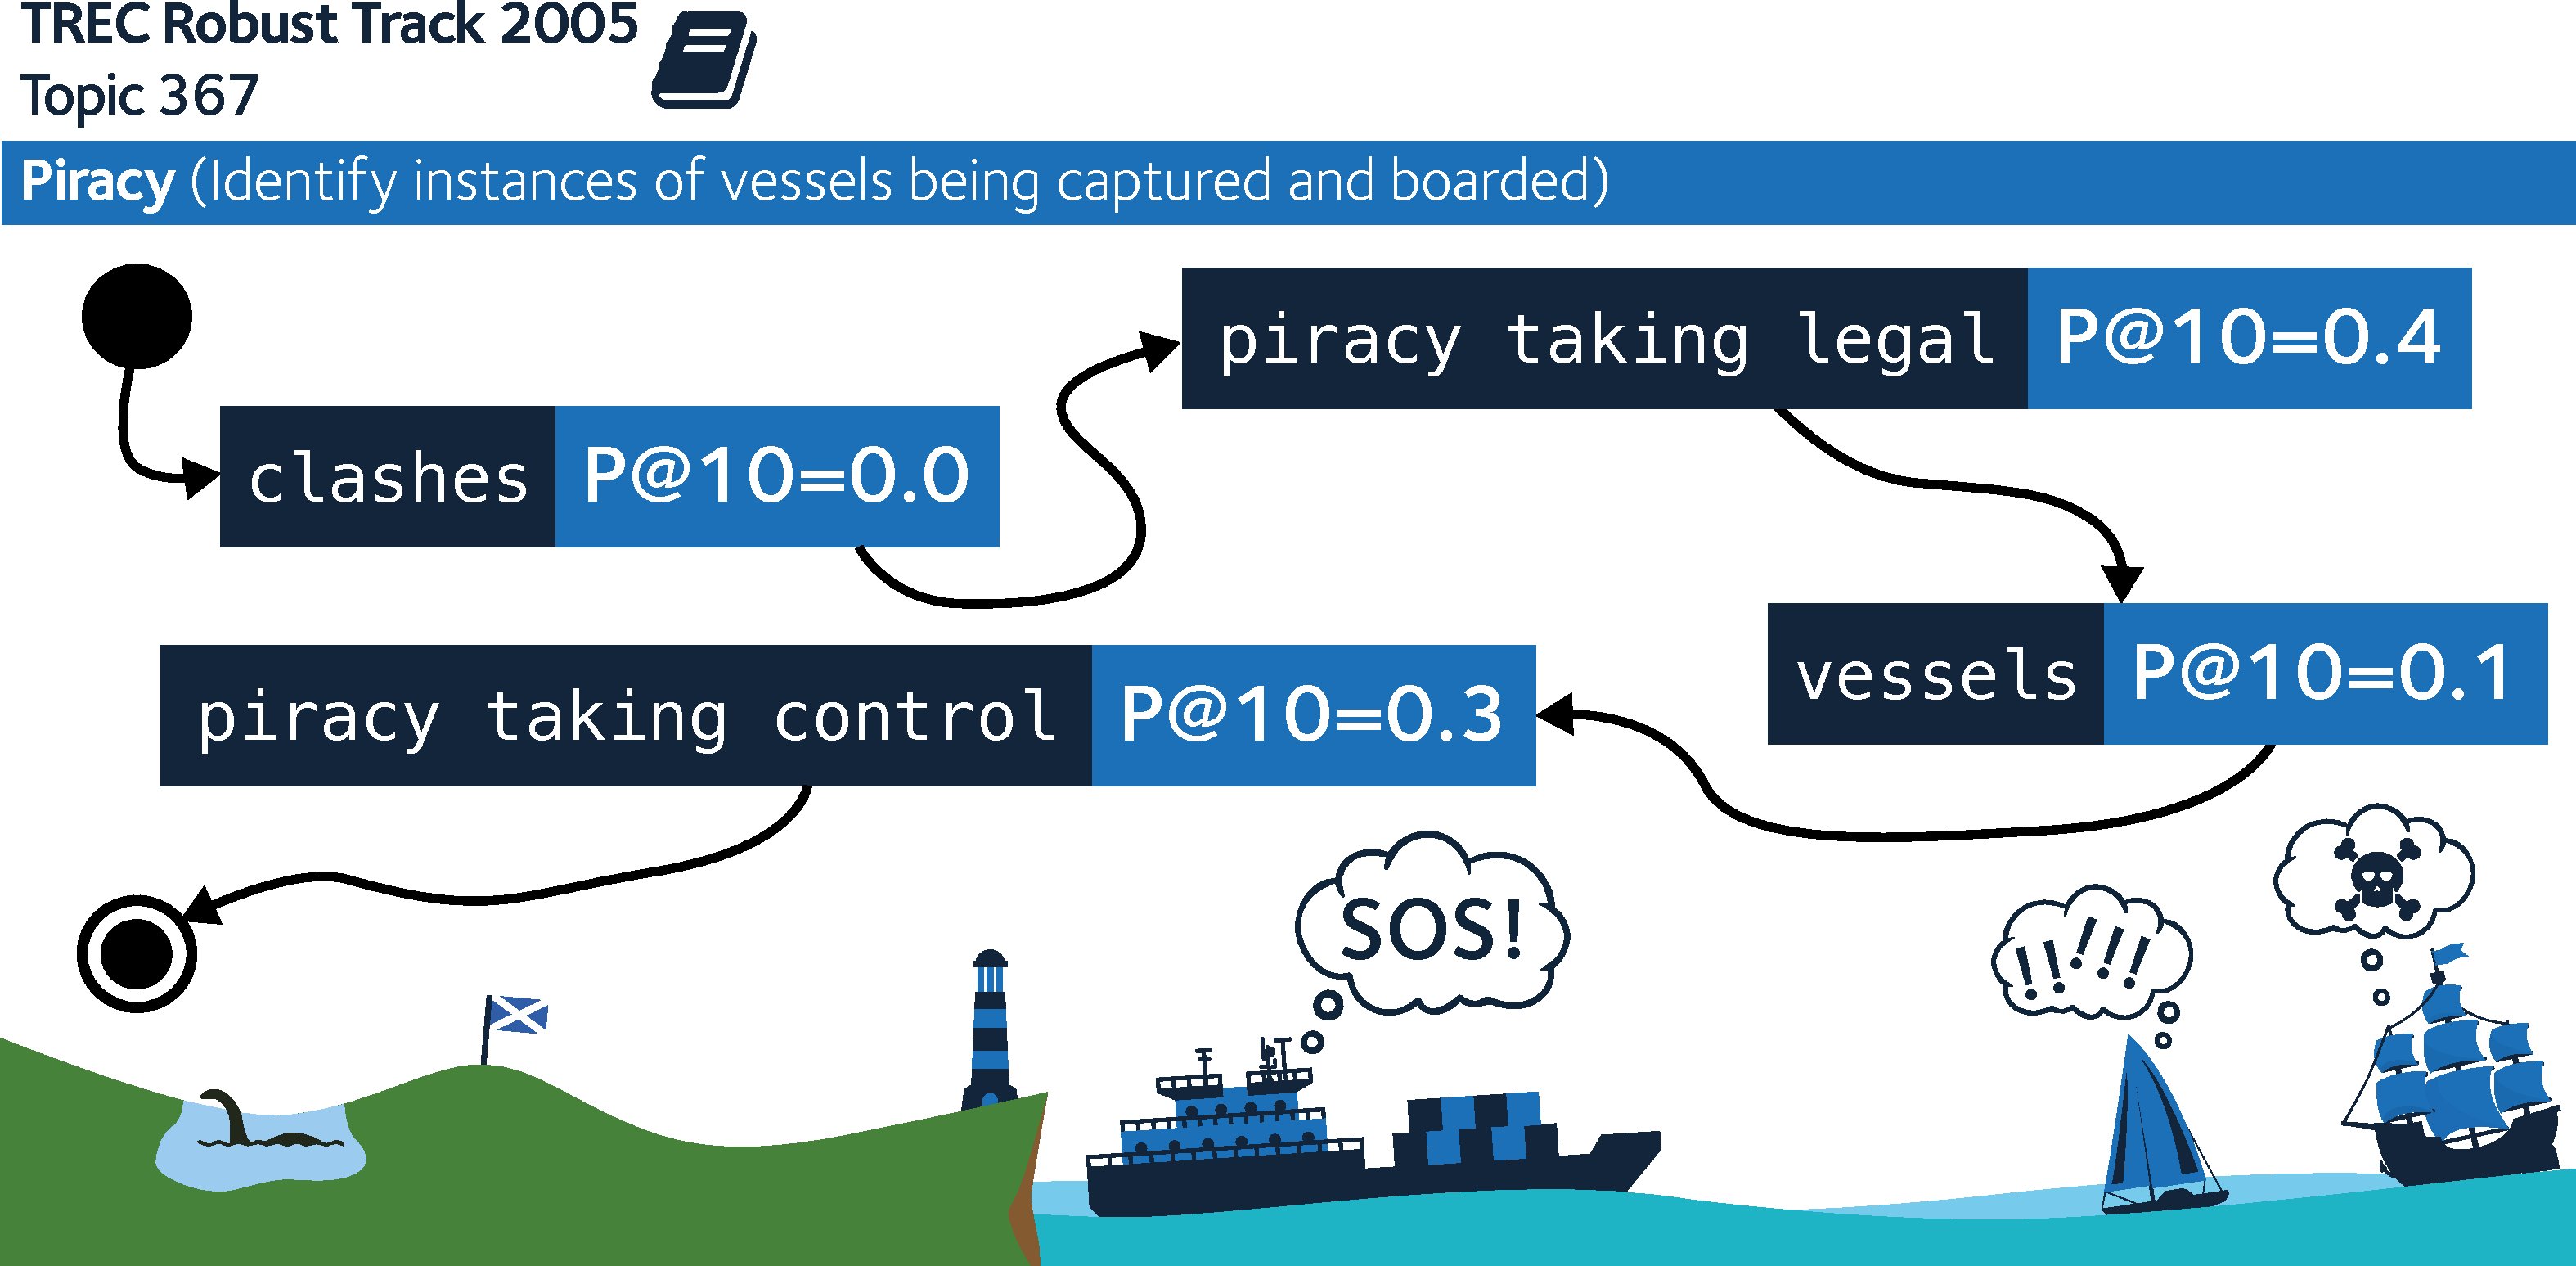
\includegraphics{figures/ch7-queries.pdf}}
    \caption[Example queries issued]{Illustration highlighting several queries issued during the performance \emph{(what-if)} experiments, generated by \blueboxbold{QS13}. The selected topic illustrated is~\gls{acr:trec} topic 367, \emph{piracy.} Notice the interleaving between single term and three term queries, along with the varying levels of performance, denoted by \emph{P@10}.}
    \label{fig:ch7_example_queries}
\end{figure}

Satisfied with the mean performance of the generated queries, we now turn our attention to the main results of the performance simulations. We primarily consider \darkblueboxbold{HL-RQ3a} in our reporting, which requires an examination of the performance for each result summary level stopping strategy. Before this however, we consider the general trends that we observed from the results of the experiments, and consider the difference between the four experimental interfaces examined.

Figure~\ref{fig:ch7_sim_perf_plots} provides twelve individual plots, one per result summary level stopping strategy. The plots represent the mean levels of performance attained at varying depths per query, averaged over the five individual topic and 50 individual trials. The mean depth per query is represented along the \emph{x} axis, with the performance attained (represented as~\gls{acr:cg}) represented on the \emph{y} axis. Although some stopping strategies caused simulated searchers to browse to depths greater than $25$ on average, we cut all plots at this value for consistency, and to better illustrate how performance varies at shallower depths.

\begin{figure}[p!]
    \centering
    \resizebox{1\hsize}{!}{
    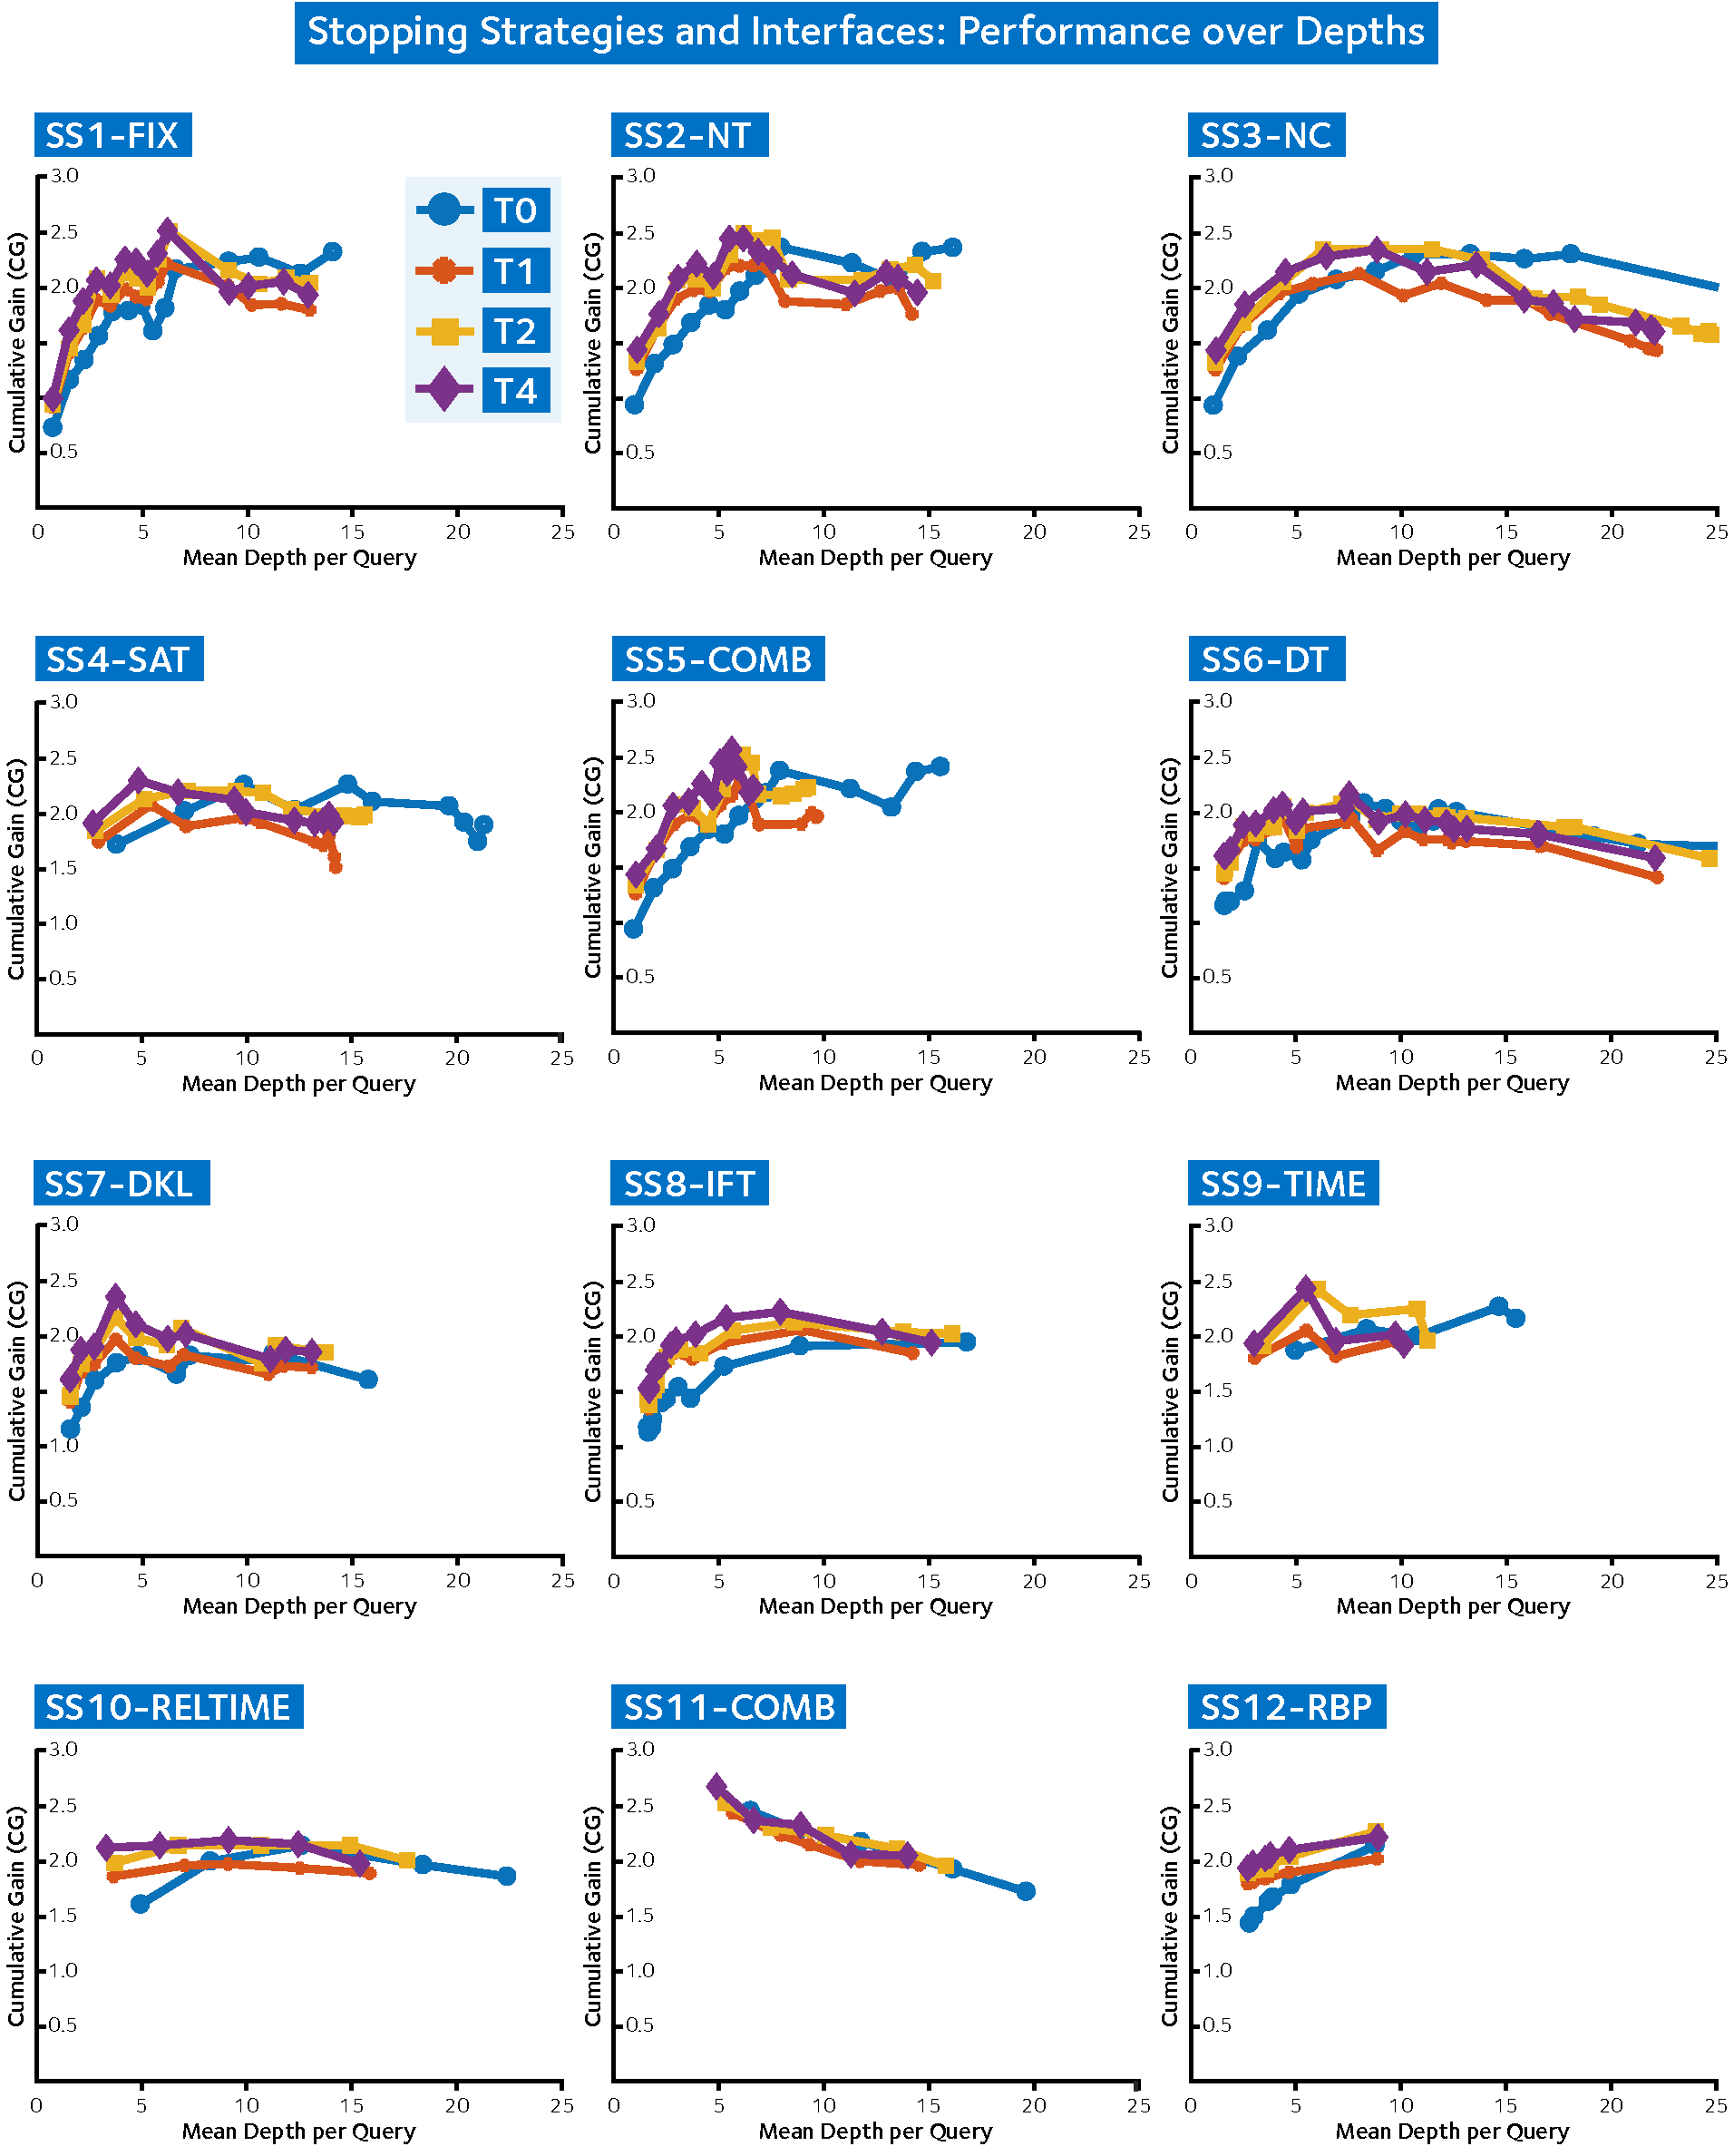
\includegraphics{figures/ch7-perf_plots.pdf}}
    \caption[Stopping strategies, interfaces and \emph{what-if} performance]{Plots showing the varying levels of performance, measured in~\gls{acr:cg}, over the mean depth per query. Each result summary stopping strategy is shown on an individual plot, with each of the four experimental interfaces shown within each plot. The depth per query reported on each \emph{x} axis is cut at 25 to allow for an easier comparison between different stopping strategies.}
    \label{fig:ch7_sim_perf_plots}
\end{figure}

General trends across all twelve strategies can be observed from the plots in Figure~\ref{fig:ch7_sim_perf_plots}. We first note that as we alter the various stopping threshold values that we trialled, we see that mean performance is attained from shallower to greater depths per query. In turn, this generally results in a gain in overall performance, with the mean~\gls{acr:cg} attained generally increasing as the depth per query increases. However, this is true only until a certain point, representing the maximum level of mean~\gls{acr:cg} attained. After this point, which is illustrated in a more profound way with some stopping strategies than others, a simulated searcher would begin to browse to greater depths on average. At greater depths, the searcher would encounter fewer and fewer potentially relevant documents, and thus would begin to waste time examining the same~\gls{acr:serp}. This is represented in the plots as the downward trend on mean~\gls{acr:cg} at greater depths per query, clearly visible after the highest level of~\gls{acr:cg} is attained. This general trend can be clearly observed from our baseline, fixed-depth stopping strategy, approximately at \dualbluebox{SS1-FIX}{@6}. An increase in mean~\gls{acr:cg} up until this depth (for most interfaces) can be observed; after this point, we observed a gradual drop-off in performance.

Considering the four plots in Figure~\ref{fig:ch7_sim_perf_plots} from the perspective of the four experimental interfaces, little difference can be observed across all twelve stopping strategies, and across the varying depths per query. The same general trends can be observed across \blueboxbold{T0}, \blueboxbold{T1}, \blueboxbold{T2} and \blueboxbold{T4}. However, some interesting observations can be made. Even though the mean levels of~\gls{acr:cg} are all very similar, we do find that interfaces yielding snippet text of greater length (interfaces \blueboxbold{T2} and \blueboxbold{T4}) generally outperform the interfaces with minimal and no snippets (interfaces \blueboxbold{T1} and \blueboxbold{T0}, respectively). This is an unsurprising result -- performance of subjects in interface \blueboxbold{T0} was generally worse in the reported user study, and this poorer performance had a subsequent impact upon the simulations of interaction which were grounded by interaction data from said user study.\footnote{Refer to Table~\ref{tbl:snippets_simulation_probcosts} for the different interaction costs and probabilities used to ground the simulations.} However, as the mean depth per query increases, we find in all plots reported in Figure~\ref{fig:ch7_sim_perf_plots} that the mean level of~\gls{acr:cg} begins to close up over each of the four interfaces. This perhaps can be attributed to the fact that at greater depths, the likelihood of encountering relevant material diminishes -- thus the gain acquired at these depths -- over all four interfaces -- begins to converge. Generally though, results are consistent across the four experimental interfaces.

\begin{table}[p!]
    \caption[Maximum CG from result summary performance runs]{Results from the simulated what-if simulated performance runs, showing the highest levels of~\gls{acr:cg} attained for each result summary level stopping strategy trialled. \emph{x\textsubscript{n}} denotes the parameter threshold(s), with \emph{DQ} denoting the depth per query at which the greatest~\gls{acr:cg} value was attained at. For each interface, the stopping strategy which attained the highest level of~\gls{acr:cg} is \darkbluebox{highlighted}. \cellbluebox{Light blue} highlighting denotes \emph{no significant difference} from the best performing strategy, with no highlighting denoting a significant difference at $\alpha$\emph{=0.05.} For combination thresholds, \emph{x\textsubscript{2},x\textsubscript{4}} are presented for \blueboxbold{SS5-COMB}, with \emph{x\textsubscript{10},x\textsubscript{4}} for \blueboxbold{SS11-COMB}.}
    \label{tbl:ch7_sim_perf}
    \renewcommand{\arraystretch}{1.8}
    \begin{center}
        \begin{tabulary}{\textwidth}{L{0.00cm}@{\CS}L{1cm}@{\CS}D{0.64cm}@{\CS}D{0.64cm}@{\CS}D{0.64cm}@{\CSONEHALF}D{0.64cm}@{\CS}D{0.64cm}@{\CS}D{0.64cm}@{\CSONEHALF}D{0.64cm}@{\CS}D{0.64cm}@{\CS}D{0.64cm}@{\CSONEHALF}D{0.64cm}@{\CS}D{0.64cm}@{\CS}D{0.64cm}@{\CS}}
            
            & & \multicolumn{3}{@{\hskip 0pt}c@{\CSONEHALF}}{\dbluecell\small\textbf{T0}} & \multicolumn{3}{@{\hskip 0pt}c@{\CSONEHALF}}{\dbluecell\small\textbf{T1}} & \multicolumn{3}{@{\hskip 0pt}c@{\CSONEHALF}}{\dbluecell\small\textbf{T2}} & \multicolumn{3}{@{\hskip 0pt}c@{\CS}}{\dbluecell\small\textbf{T4}}\\
            
            \RS & & \lbluecell\small\textbf{x\textsubscript{n}} & \lbluecell\small\textbf{DQ} & \lbluecell\small\textbf{CG} & \lbluecell\small\textbf{x\textsubscript{n}} & \lbluecell\small\textbf{DQ} & \lbluecell\small\textbf{CG} & \lbluecell\small\textbf{x\textsubscript{n}} & \lbluecell\small\textbf{DQ} & \lbluecell\small\textbf{CG} & \lbluecell\small\textbf{x\textsubscript{n}} & \lbluecell\small\textbf{DQ} & \lbluecell\small\textbf{CG} \\
            
            \RS \multirow{1}{*}{\hspace*{-2mm}\rotatebox{90}{\hspace*{-1mm}\small\textbf{FIX}}} & \lbluecell\small\textbf{SS1} & \cell \small \hspace*{-1mm} 24 & \cell \small \hspace*{-2.5mm} 14.09 & \cell \hspace*{-1mm} \small 2.31 & \cell \small \hspace*{-1mm} 10 & \cell \small \hspace*{-1mm} 6.19 & \cell \hspace*{-1mm} \small 2.20 & \cell \small \hspace*{-1mm} 10 & \cell \small \hspace*{-1mm} 6.33 & \cell \hspace*{-1mm} \small 2.50 & \cell \small \hspace*{-1mm} 10 & \cell \small \hspace*{-1mm} 6.23 & \cell \hspace*{-1mm} \small 2.50 \\
            
            \RS\RS\RS \multirow{2}{*}{\hspace*{-2mm}\rotatebox{90}{\hspace*{-3mm}\small\textbf{FRUS}}} & \lbluecell\small\textbf{SS2} & \cell \small \hspace*{-1mm} 10 & \cell \small \hspace*{-1mm} 7.94 & \cell \hspace*{-1mm} \small 2.36 & \cell \small \hspace*{-1mm} 8 & \cell \small \hspace*{-1mm} 6.61 & \cell \hspace*{-1mm} \small 2.20 & \cell \small \hspace*{-1mm} 7 & \cell \small \hspace*{-1mm} 6.16 & \cell \hspace*{-1mm} \small 2.49 & \cell \small \hspace*{-1mm} 6 & \cell \small \hspace*{-1mm} 5.49 & \cell \hspace*{-1mm} \small 2.44 \\
            
            \RS & \lbluecell\small\textbf{SS3} & \cell \small \hspace*{-1mm} 8 & \cell \small \hspace*{-2.5mm} 13.22 & \cell \hspace*{-1mm} \small 2.31 & \cell \small \hspace*{-1mm} 5 & \cell \small \hspace*{-1mm} 7.91 & \cell \hspace*{-1mm} \small 2.13 & \cell \small \hspace*{-1mm} 4 & \cell \small \hspace*{-1mm} 6.19 & \cell \hspace*{-1mm} \small 2.35 & \cell \small \hspace*{-1mm} 5 & \cell \small \hspace*{-1mm} 8.76 & \cell \hspace*{-1mm} \small 2.35 \\
            
            \RS\RS\RS \multirow{1}{*}{\hspace*{-2mm}\rotatebox{90}{\small\textbf{SAT}}} & \lbluecell\small\textbf{SS4} & \cell \small \hspace*{-1mm} 5 & \cell \small \hspace*{-2.5mm} 14.79 & \cell \hspace*{-1mm} \small 2.26 & \cell \small \hspace*{-1mm} 2 & \cell \small \hspace*{-1mm} 5.40 & \cell \hspace*{-1mm} \small 2.08 & \cell \small \hspace*{-1mm} 3 & \cell \small \hspace*{-1mm} 7.15 & \cell \hspace*{-1mm} \small 2.21 & \cell \small \hspace*{-1mm} 2 & \cell \small \hspace*{-1mm} 4.80 & \cell \hspace*{-1mm} \small 2.30 \\
            
            \RS\RS\RS \multirow{1}{*}{\hspace*{-2mm}\rotatebox{90}{\small\textbf{COM}}} & \lbluecell\small\textbf{SS5} & \cell \small \hspace*{-1mm} 24,8 & \cell \small \hspace*{-2.5mm} 15.58 & \cell \hspace*{-1mm} \small 2.41 & \cell \small \hspace*{-1mm} 8,4 & \cell \small \hspace*{-1mm} 6.05 & \cell \hspace*{-1mm} \small 2.30 & \cell \small \hspace*{-1mm} 8,4 & \cell \small \hspace*{-1mm} 6.17 & \cell \hspace*{-1mm} \small 2.52 & \cell \small \hspace*{-1mm} 9,3 & \cell \small \hspace*{-1mm} 5.65 & \cell \hspace*{-1mm} \small 2.56 \\
            
            \RS\RS\RS \multirow{2}{*}{\hspace*{-2mm}\rotatebox{90}{\small\textbf{DIFF}}} & \lbluecell\small\textbf{SS6} & \cell \small \hspace*{-1mm} 0.55 & \cell \small \hspace*{-1mm} 8.23 & \cell \hspace*{-1mm} \small 2.08 & \small \hspace*{-1mm} 0.35 & \small \hspace*{-1mm} 4.35 & \hspace*{-1mm} \small 1.96 & \cell \small \hspace*{-1mm} 0.55 & \cell \small \hspace*{-1mm} 7.48 & \cell \hspace*{-1mm} \small 2.12 & \small \hspace*{-1mm} 0.55 & \small \hspace*{-1mm} 7.53 & \hspace*{-1mm} \small 2.16 \\
            
            \RS & \lbluecell\small\textbf{SS7} & \small \hspace*{-1mm} 3.5 & \small \hspace*{-2.5mm} 11.24 & \hspace*{-1mm} \small 1.84 & \small \hspace*{-1mm} 6.0 & \small \hspace*{-1mm} 3.73 & \hspace*{-1mm} \small 1.97 & \cell \small \hspace*{-1mm} 6.0 & \cell \small \hspace*{-1mm} 3.71 & \cell \hspace*{-1mm} \small 2.16 & \cell \small \hspace*{-1mm} 6.0 & \cell \small \hspace*{-1mm} 3.72 & \cell \hspace*{-1mm} \small 2.35 \\
            
            \RS\RS\RS \multirow{1}{*}{\hspace*{-2mm}\rotatebox{90}{\small\textbf{IFT}}} & \lbluecell\small\textbf{SS8} & \small \hspace*{-2.5mm} 0.002 & \small \hspace*{-2.5mm} 16.83 & \hspace*{-1mm} \small 1.95 & \cell \small \hspace*{-2.5mm} 0.004 & \cell \small \hspace*{-1mm} 8.96 & \cell \hspace*{-1mm} \small 2.06 & \cell \small \hspace*{-2.5mm} 0.006 & \cell \small \hspace*{-1mm} 8.59 & \cell \hspace*{-1mm} \small 2.13 & \cell \small \hspace*{-2.5mm} 0.006 & \cell \small \hspace*{-1mm} 7.93 & \cell \hspace*{-1mm} \small 2.23 \\
            
            \RS\RS\RS \multirow{2}{*}{\hspace*{-2mm}\rotatebox{90}{\hspace*{-2mm}\small\textbf{TIME}}} & \lbluecell\small\textbf{SS9} & \cell \small \hspace*{-1mm} 120 & \cell \small \hspace*{-2.5mm} 14.61 & \cell \hspace*{-1mm} \small 2.27 & \cell \small \hspace*{-1mm} 60 & \cell \small \hspace*{-1mm} 5.43 & \cell \hspace*{-1mm} \small 2.05 & \cell \small \hspace*{-1mm} 60 & \cell \small \hspace*{-1mm} 5.95 & \cell \hspace*{-1mm} \small 2.42 & \cell \small \hspace*{-1mm} 60 & \cell \small \hspace*{-1mm} 5.41 & \cell \hspace*{-1mm} \small 2.43 \\
            
            \RS & \lbluecell\small\textbf{SS10} & \cell \small \hspace*{-1mm} 30 & \cell \small \hspace*{-2.5mm} 12.60 & \cell \hspace*{-1mm} \small 2.14 & \small \hspace*{-1mm} 30 & \small \hspace*{-1mm} 9.09 & \hspace*{-1mm} \small 1.98 & \cell \small \hspace*{-1mm} 20 & \cell \small \hspace*{-1mm} 6.73 & \cell \hspace*{-1mm} \small 2.14 & \small \hspace*{-1mm} 30 & \small \hspace*{-1mm} 9.12 & \hspace*{-1mm} \small 2.19 \\
            
            \RS\RS\RS \multirow{1}{*}{\hspace*{-2mm}\rotatebox{90}{\small\textbf{COM}}} & \lbluecell\small\textbf{SS11} & \dbluecell \small \hspace*{-1mm} 10,8 & \dbluecell \small \hspace*{-1mm} 6.53 & \dbluecell \hspace*{-1mm} \small 2.45 & \dbluecell \small \hspace*{-2.5mm} 10,10 & \dbluecell \small \hspace*{-1mm} 5.66 & \dbluecell \hspace*{-1mm} \small 2.44 & \dbluecell \small \hspace*{-2.5mm} 10,10 & \dbluecell \small \hspace*{-1mm} 5.33 & \dbluecell \hspace*{-1mm} \small 2.52 & \dbluecell \small \hspace*{-2.5mm} 10,10 & \dbluecell \small \hspace*{-1mm} 4.91 & \dbluecell \hspace*{-1mm} \small 2.67 \\
            
            \RS\RS\RS \multirow{1}{*}{\hspace*{-2mm}\rotatebox{90}{\small\textbf{RBP}}} & \lbluecell\small\textbf{SS12} &  \small \hspace*{-1mm} 0.99 & \small \hspace*{-1mm} 8.78 & \hspace*{-1mm} \small 2.15 & \small \hspace*{-1mm} 0.99 & \small \hspace*{-1mm} 8.87 & \hspace*{-1mm} \small 2.03 & \cell \small \hspace*{-1mm} 0.99 & \cell \small \hspace*{-1mm} 8.81 & \cell \hspace*{-1mm} \small 2.27 & \small \hspace*{-1mm} 0.99 & \small \hspace*{-1mm} 8.90 & \hspace*{-1mm} \small 2.22 \\
            
        \end{tabulary}
        \end{center}
    \end{table}

With the twelve plots in Figure~\ref{fig:ch7_sim_perf_plots} presenting a broad overview of the variation in performance as the mean depth per query increases, we now turn our attention to the peaks in each plot for the four individual experimental interfaces -- or the \emph{highest levels of~\gls{acr:cg} that are attained.} Table~\ref{tbl:ch7_sim_perf} reports these values, across each of the twelve stopping strategies (rows), and over the four individual experimental interfaces (columns, grouped by \blueboxbold{T0}, \blueboxbold{T1}, \blueboxbold{T2} or \blueboxbold{T4}). For each of the twelve stopping strategies, we report: the highest level of~\gls{acr:cg} attained (\genericblack{CG}); the mean depth per query at which this value was reached (\genericblack{DQ}); and the stopping threshold value(s) used to reach this value (\genericblack{x\textsubscript{n}}). \darkbluebox{Highlighted} are the stopping strategies that yielded the greatest overall level of~\gls{acr:cg}. Across all four interfaces, combination stopping strategy \blueboxbold{SS11-COMB} attained this, with mean~\gls{acr:cg} values of $2.45$, $2.44$, $2.52$ and $2.67$ reported for interfaces \blueboxbold{T0}, \blueboxbold{T1}, \blueboxbold{T2} and \blueboxbold{T4} respectively. These values were all reached at similar depths per query ($\~5-6.5$), and with a similar range of threshold values, with $x_4\approx8-10$, and $x_{10}=10$ seconds.\footnote{As a reminder, \blueboxbold{SS11-COMB} considers the type of patch presented by a given~\gls{acr:serp}, before employing either the satisfaction-based stopping strategy \blueboxbold{SS4-SAT} for high yields early on, or the give-up time-based stopping strategy \blueboxbold{SS10-RELTIME} if the~\gls{acr:serp} does not appear to yield promising results early on.} The relatively low levels of mean depths per query ($6.53$, $5.66$, $5.33$ and $4.91$ for interfaces \blueboxbold{T0}, \blueboxbold{T1}, \blueboxbold{T2} and \blueboxbold{T4} respectively) at which the best~\gls{acr:cg} was attained also demonstrates that \blueboxbold{SS11-COMB} was particularly robust at detecting a~\gls{acr:serp} with good results, and vice versa. As such, the low depths per query indicate that the simulated searchers were confidently able to abandon poor quality~\glsplural{acr:serp} without affecting their overall performance.

\begin{table}[h!]
    \renewcommand{\arraystretch}{1.8}
    \begin{center}
        \begin{tabulary}{\textwidth}{L{3.2cm}@{\CSONEHALF}D{2.6cm}@{\CSONEHALF}D{2.6cm}@{\CSONEHALF}D{2.6cm}@{\CSONEHALF}D{2.6cm}@{\CS}}
            & \lbluecell\small\textbf{T0} & \lbluecell\small\textbf{T1} & \lbluecell\small\textbf{T2} & \lbluecell\small\textbf{T4}\\
            
            \RS \lbluecell\small\textbf{SS5-COMB} & \cell\small 2.41$\pm$2.47 & \cell\small 2.30$\pm$2.44 & \cell\small 2.52$\pm$2.67 & \cell\small 2.56$\pm$2.27 \\
            \RS \lbluecell\small\textbf{SS11-COMB} & \cell \small 2.45$\pm$2.59 & \cell\small 2.44$\pm$2.41 & \cell\small 2.52$\pm$2.52 & \cell\small 2.67$\pm$2.52 \\
        \end{tabulary}
        \end{center}
    \end{table}

Upon closer examination of Table~\ref{tbl:ch7_sim_perf}, we also find that the other combination strategy \blueboxbold{SS5-COMB} (relating to a combination of both frustration and satisfaction stopping strategies) consistently placed second in performance rankings across the four experimental interfaces trialled, very close behind the mean~\gls{acr:cg} values attained by \blueboxbold{SS11-COMB} (with mean~\gls{acr:cg} values $\pm$ standard deviations for both combination strategies reported in the small table above). Again, this demonstrates that a combination strategy appears to be very effective at eliciting good levels of performance, and suggests that a degree of flexibility in selecting their stopping criterion/criteria is advantageous to searchers. However, these levels of~\gls{acr:cg} were attained over much higher mean depths per query than the other combination strategy counterpart ($14.76$, $16.45$, $15.22$ and $14.58$ for interfaces \blueboxbold{T0}, \blueboxbold{T1}, \blueboxbold{T2} and \blueboxbold{T4} respectively). Over interface \blueboxbold{T0} especially, a high number of non-relevant documents were required to be found ($24$) before stopping.

\begin{figure}[t!]
    \centering
    \resizebox{1\hsize}{!}{
    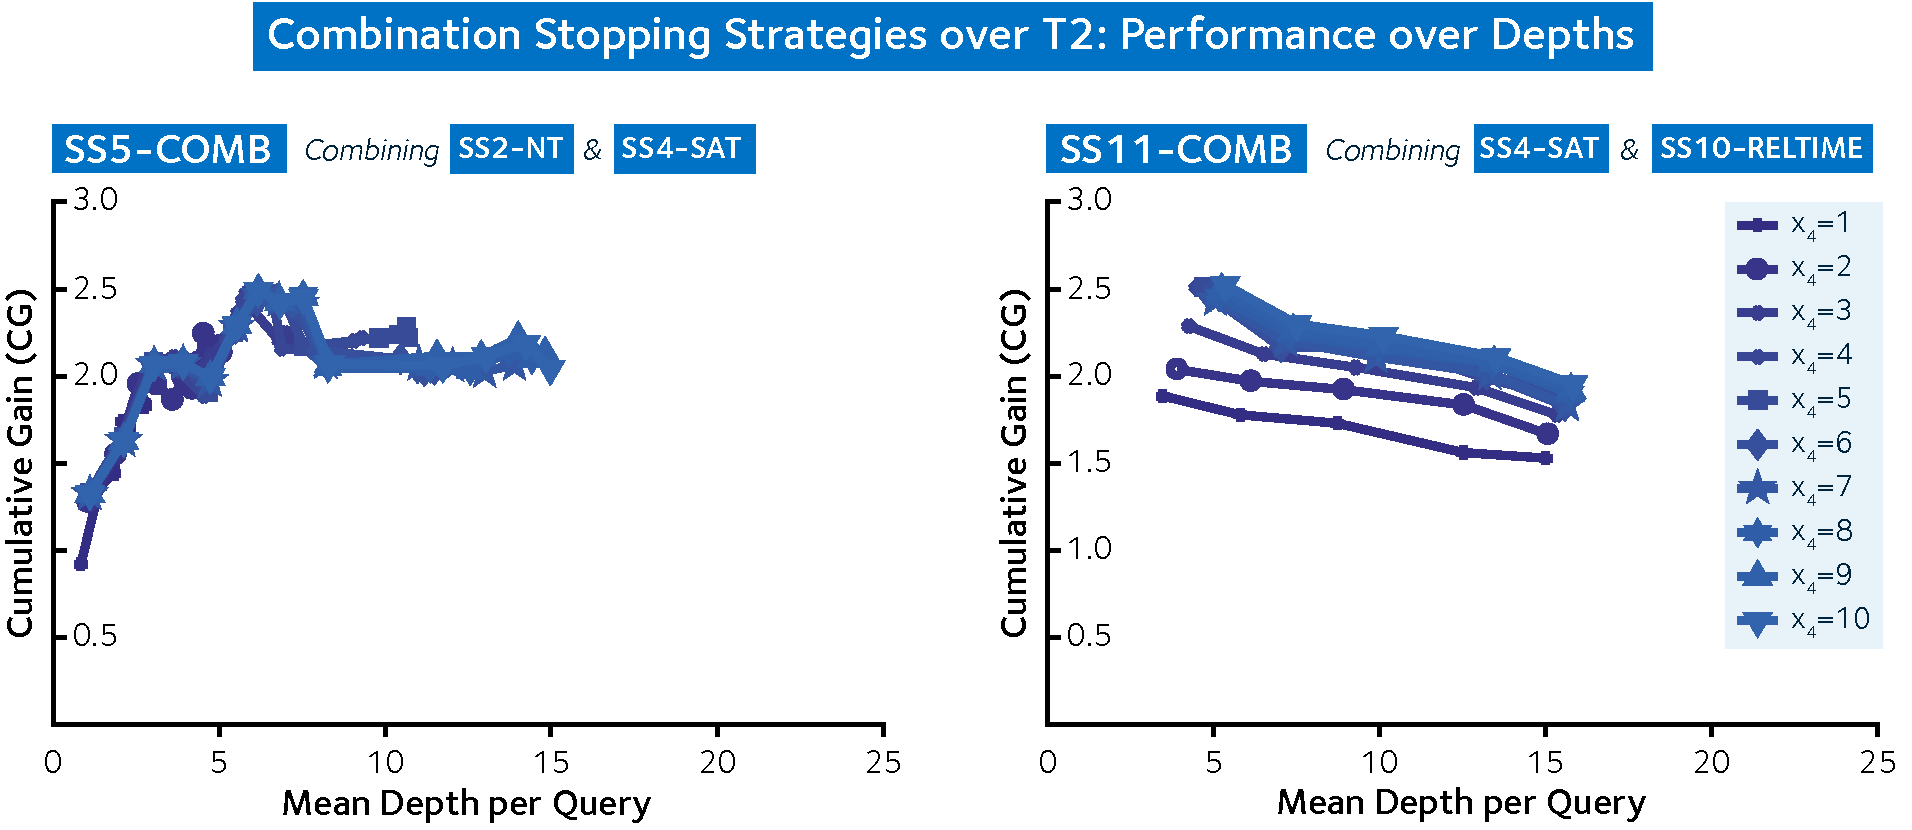
\includegraphics{figures/ch7-perf_plots_combo.pdf}}
    \caption[\emph{What-if} performance over combination stopping strategies]{Plots illustrating performance over varying depths per query. Reported are performance values over combination strategies \blueboxbold{SS5-COMB} (left) and \blueboxbold{SS11-COMB} (right). With each line representing a value from \emph{x\textsubscript{4}} (refer to legend), each point on the lines represents performance and depth for a threshold value from \emph{x\textsubscript{2}} on the left, and \emph{x\textsubscript{10}} on the right. Little difference in performance is observed between variations of parameter combinations.}
    \label{fig:ch7_sim_perf_plots_combo}
\end{figure}

It should be noted that the two plots reported in Figure~\ref{fig:ch7_sim_perf_plots} for both \blueboxbold{SS5-COMB} and \blueboxbold{SS11-COMB} are shown over the best performing $x_4$ value for each stopping strategy, as reported in Table~\ref{tbl:ch7_sim_perf}. With two sets of parameters for these combination strategies, reporting in these plots would have been cumbersome -- Figure~\ref{fig:ch7_sim_perf_plots_combo} instead reports the varying levels of~\gls{acr:cg} across different mean depths per query, for each of the different $x_4$ values trialled. These are shown over interface \blueboxbold{T2} only; similar plots were observed for the other three experimental interfaces, yet are not reported. We can see from these plots that similar trends can be observed across the range of mean depths per query across both stopping strategies. The change in performance for \blueboxbold{SS11-COMB} is more profound -- as $x_4$ increases, so too does the mean level of~\gls{acr:cg} attained.

With both \blueboxbold{SS5-COMB} and \blueboxbold{SS11-COMB} both performing very well in terms of the highest levels of~\gls{acr:cg} attained, a cursory examination of Table~\ref{tbl:ch7_sim_perf} will also confirm that several other strategies also perform to a high standard. With these generally high levels of performance being reported, we decided to perform statistical significance testing to determine if the performance of any stopping strategies were sufficiently different from that of \blueboxbold{SS11-COMB}. As discussed previously in this section, we performed two-tailed Student's t-tests over the~\gls{acr:cg} values, comparing \blueboxbold{SS11-COMB} against the other eleven stopping strategies. Results of the statistical testing showed that a majority of stopping strategies were indeed \emph{not significant} ($p>0.05$), denoting that the performance was similar to \blueboxbold{SS11-COMB}. In Table~\ref{tbl:ch7_sim_perf}, \cellbluebox{cells highlighted} denote that the represented stopping strategy was similar in terms of performance to the best performing. Stopping strategies without any cell highlighting offered statistically significant differences, meaning that~\gls{acr:cg} were sufficiently worse than those of \blueboxbold{SS11-COMB}. Of the eleven remaining stopping strategies, we generally observe -- across the four interfaces -- that the following showed similar levels of performance:

\begin{itemize}
    \item{\blueboxbold{SS1-FIX}, the fixed-depth stopping strategy;}
    \item{\blueboxbold{SS2-NT} and \blueboxbold{SS3-NC}, the frustration-based strategies;}
    \item{\blueboxbold{SS4-SAT}, the satiation-based stopping strategy;}
    \item{\blueboxbold{SS5-COMB}, the frustration and satiation combination strategy;}
    \item{\blueboxbold{SS8-IFT}, the~\gls{acr:ift}-based stopping strategy; and}
    \item{\blueboxbold{SS9-TIME} and \blueboxbold{SS10-RELTIME}, the time-based stopping strategies.}
\end{itemize}

This accounts for a majority of the remaining eleven stopping strategies trialled. The remaining three:

\begin{itemize}
    \item{\blueboxbold{SS6-DT} and \blueboxbold{SS7-DKL}, the difference-based stopping strategies; and}
    \item{\blueboxbold{SS12-RBP}, the~\gls{acr:rbp}-based stopping strategy}
\end{itemize}

\noindent
generally offered significantly different levels of~\gls{acr:cg} (across the four experimental interfaces) from those of \blueboxbold{SS11-COMBO}. We now briefly examine the undiscussed stopping strategies, before moving to the reporting of the real-world simulated comparisons.

We first consider \blueboxbold{SS1-FIX}, \blueboxbold{SS2-NT} and \blueboxbold{SS3-NC} together. Examining the figures for the first three stopping strategies in Figure~\ref{fig:ch7_sim_perf_plots}, we observe very similar plots following the aforementioned trends in mean performance over mean depths per query. Comparing the plots for \blueboxbold{SS1-FIX} and \blueboxbold{SS2-NT} in particular, striking similarities can be observed. \blueboxbold{SS3-NC} yields similar plots, but spread over greater mean depths per query.\footnote{This is due to the fact that the stopping criterion for \blueboxbold{SS3-NC} considers a series of contiguous, non-relevant items to be found. This can mean that a searcher subscribing to this stopping strategy will examine content to greater depths before meeting this criterion.} Examining Table~\ref{tbl:ch7_sim_perf}, similar levels of~\gls{acr:cg} can also be attained over three stopping strategies, all at similar mean depths per query ($2.50$ at a D/Q of $6.33$, $2.49$ at a D/Q of $6.16$ and $2.35$ at a D/Q of $6.19$ for \blueboxbold{SS1-FIX}, \blueboxbold{SS2-NT} and \blueboxbold{SS3-NC} respectively, over interface \blueboxbold{T2}). This result is interesting as intuitively, both \blueboxbold{SS2-NT} and \blueboxbold{SS3-NC} should offer greater performance over \blueboxbold{SS1-FIX}. This is because the frustration-based stopping strategies are \emph{adapative} in nature, curtailing the examination of result summaries early when results are mostly non-relevant. This is in contrast to the fixed-depth strategy (and baseline) of \blueboxbold{SS1-FIX}.

Moving to the satiation-based stopping strategy \blueboxbold{SS4-SAT}, we find that the associated plot in Figure~\ref{fig:ch7_sim_perf_plots} looks somewhat invariant compared to other strategies. A relatively consistent level of~\gls{acr:cg} can be attained at a range of mean depths per query. It is somewhat surprising how this stopping strategy performs so well, given that it may have been better suited to a session-based stopping decision point (e.g. as applied in the study reported in Chapter~\ref{chap:diversity}) than being applied at the result summary level. Nevertheless, \blueboxbold{SS4-SAT} yields good levels of~\gls{acr:cg} ($2.10-2.30$). A low stopping threshold value ranging from $2$ to $5$ provides these levels of~\gls{acr:cg} across the four experimental interfaces.

Turning our attention to the~\gls{acr:ift}-based stopping strategy \blueboxbold{SS8-IFT}, we notice the lower values of~\gls{acr:cg} that are attained in Table~\ref{tbl:ch7_sim_perf}. These values are generally attained at greater mean depths per query, and if we examine the plot for \blueboxbold{SS8-IFT} in Figure~\ref{fig:ch7_sim_perf_plots}, we notice a definite drop in mean accumulated~\gls{acr:cg} after this peak. However, the low levels of~\gls{acr:cg} in comparison to other stopping strategies (e.g. $2.13$ vs. $2.52$ for \blueboxbold{SS11-COMB} over interface \blueboxbold{T2}) suggests that this approach does not work particularly well. This perhaps can be attributed to how the \emph{rate of gain} was calculated -- a difficult value to estimate. We discuss the issue of calculating the rate of gain a searcher would expect to accrue in greater detail  in our discussion chapter, Chapter~\ref{chap:conclusions}.

We next consider the time-based stopping strategies, \blueboxbold{SS9-TIME} and \blueboxbold{SS10-RELTIME}. The first stopping strategy can be considered analogous to a fixed-depth approach, considering the time from the point at which a~\gls{acr:serp} is presented. The second strategy can be considered more adaptive, considering the time from which the last relevant document was saved). To this end, it is a somewhat interesting result that \blueboxbold{SS9-TIME} consistently yields a higher level of~\gls{acr:cg} across all four experimental interfaces ($2.27$, $2.05$, $2.42$ and $2.43$ for \blueboxbold{T0}, \blueboxbold{T1}, \blueboxbold{T2} and \blueboxbold{T4} respectively) than when compared to \blueboxbold{SS10-RELTIME} ($2.14$, $1.98$, $2.14$ and $2.19$ for \blueboxbold{T0}, \blueboxbold{T1}, \blueboxbold{T2} and \blueboxbold{T4} respectively -- with the~\gls{acr:cg} attained for \blueboxbold{T4} significantly different from best performing strategy, \blueboxbold{SS11-COMB}). Intuitively, one would expect higher performance to be attained by the more adaptive approach, where searchers would stop earlier when examining a poor set of results. The performance across \blueboxbold{SS10-RELTIME} is invariant across mean depths per query, as illustrated in Figure~\ref{fig:ch7_sim_perf_plots}. A smaller number of points reflects the smaller number of threshold values that we trialled. These are summarised as $x_9$ and $x_{10}$ in Table~\ref{tbl:stopping_thresholds} on page~\pageref{tbl:stopping_thresholds}.

Difference-based stopping strategies \blueboxbold{SS6-DT} and \blueboxbold{SS7-DKL} are considered next. As reported earlier, these stopping strategies offered significant differences in performance across interfaces \blueboxbold{T1} and \blueboxbold{T4} when compared to the best performing stopping strategy \blueboxbold{SS1-COMB}. Indeed, performance is generally poor in comparison to other stopping strategies that were trialled in this study. As can be seen from the performance plots in Figure~\ref{fig:ch7_sim_perf_plots} however, the greater the depth a searcher was to go on average, the better performance would be. We discuss the findings -- as well a discussion of the poor performance it yielded -- of this stopping strategy in more detail in Chapter~\ref{chap:conclusions}.

Our final stopping strategy is the~\gls{acr:rbp}-based approach, \blueboxbold{SS12-RBP}. From the plot in Figure~\ref{fig:ch7_sim_perf_plots}, it is clear that~\gls{acr:rbp} provides lower levels of~\gls{acr:cg} when compared to other stopping strategies. An intuitive result is that as the patience parameter was increased, simulated searchers would traverse to greater depths on average -- the highest levels of~\gls{acr:cg} as reported in Table~\ref{tbl:ch7_sim_perf} are attained however at greater depths on average than \blueboxbold{SS11-COMB}.

While \blueboxbold{SS11-COMB} consistently offers the highest level of~\gls{acr:cg} across the four experimental interfaces, it is clear from our results that it does not do so by a large margin -- indeed, several other stopping strategies offer maximum~\gls{acr:cg} values that are very close to that of \blueboxbold{SS11-COMB}. Indeed, this combination stopping strategy does not offer a significant improvement in performance over our fixed-depth baseline, \blueboxbold{SS1-FIX}. It does, however, offer a marginally greater level of~\gls{acr:cg} at comparatively lower depths per query on average, demonstrating that it is a more robust and efficient means for determining when to stop.

\subsubsection{Real-World Comparisons}\label{sec:snippets:simulations:results:comparisons}
From our \emph{what-if} performance simulations that examined what would happen if a particular stopping strategy were to be rigidly followed, we now examine how closely each of the aforementioned stopping strategies compare to actual searcher behaviours. As such, this provides an answer to \darkblueboxbold{HL-RQ3b} under the context of varying result summary lengths. As a reminder, these simulations \emph{replayed} all of the queries issued by real-world searchers, allowing us to compare real-world and simulated click depths.

\begin{figure}[p!]
    \centering
    \resizebox{1\hsize}{!}{
    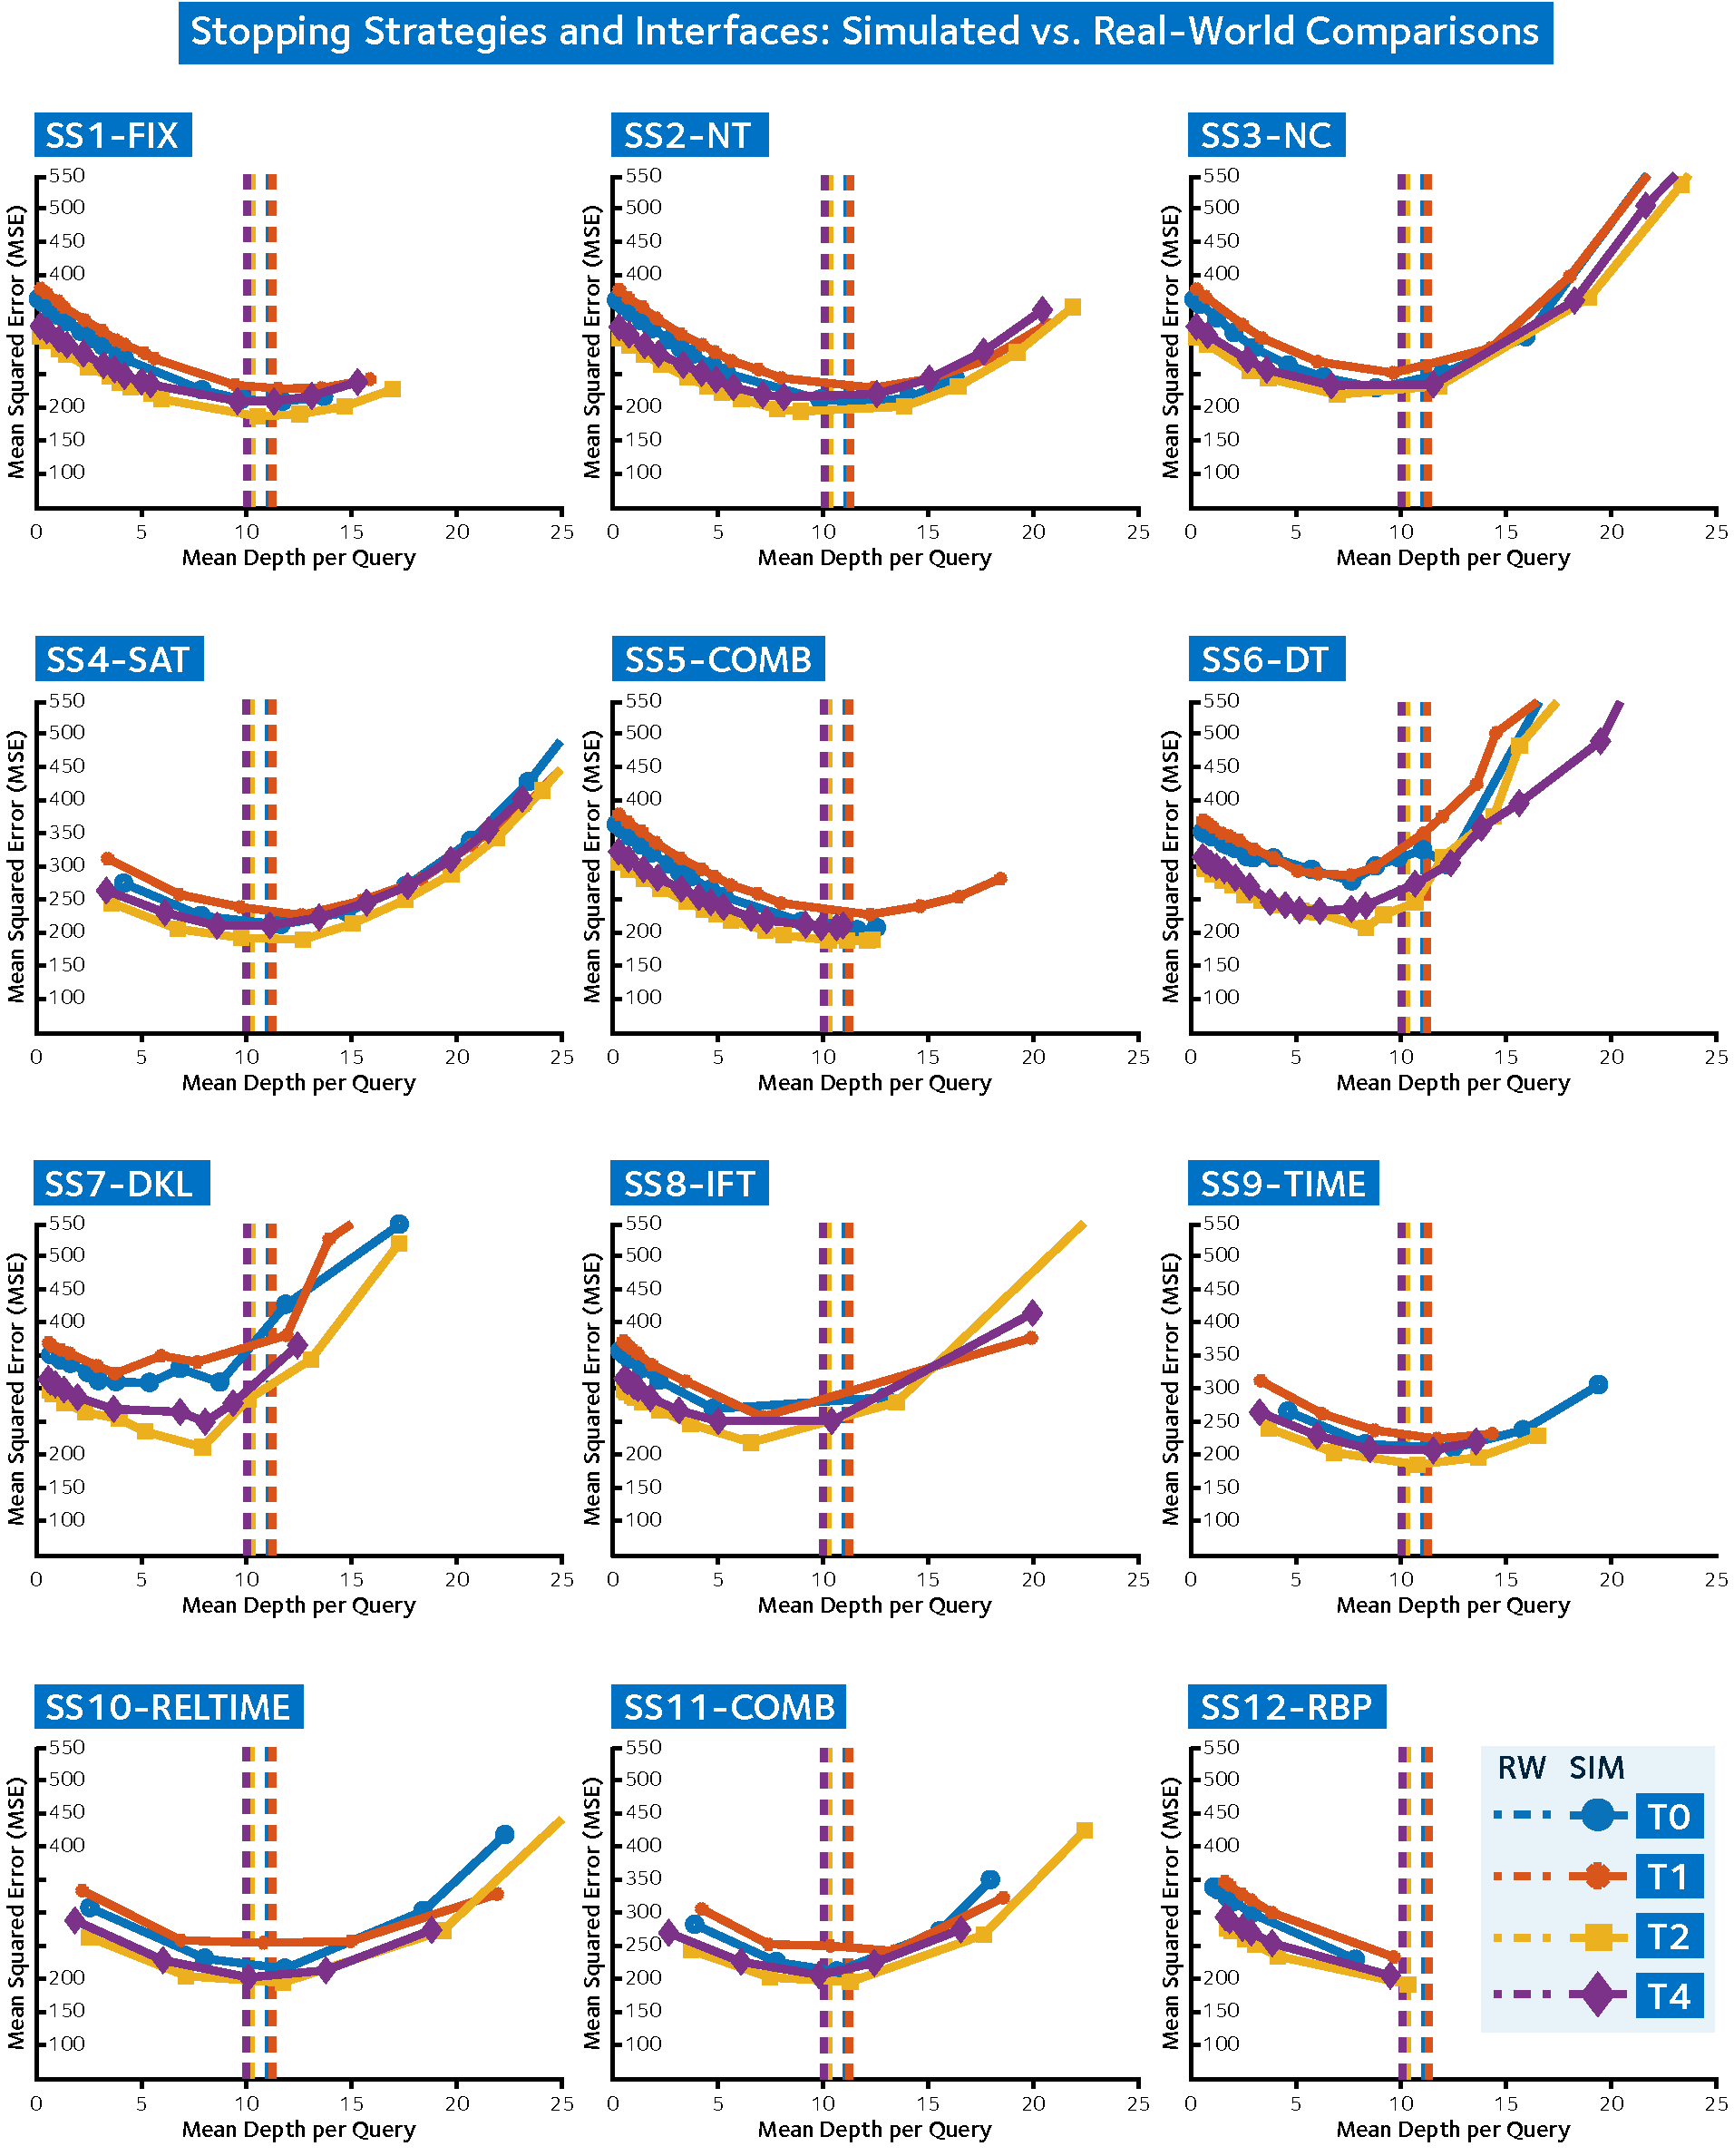
\includegraphics{figures/ch7-comparison_plots.pdf}}
    \caption[Real-world comparisons over stopping strategies]{Plots reporting the comparison runs, reporting the MSE vs. the mean depth per query. Runs over each of the four experimental interfaces are shown. Also included in the plots are a series of dashed lines denoting the mean depth per query reached by the real-world subjects of the user study. Depths per query (and mean~\gls{acr:cg} values) are also reported in Table~\ref{tbl:ch7_sim_comp_cgdq}.}
    \label{fig:ch7_sim_comparison_plots}
\end{figure}

\begin{table}[p!]
    \caption[Lowest MSE values for comparisons runs]{Results from the simulated comparison runs, showing the \emph{lowest} MSE value reached over each result summary level stopping strategy trialled (grouped by their type). \emph{x\textsubscript{n}} denotes the parameter threshold(s) that the lowest MSE was reached with. Results are presented across the four experimental interfaces, including an average over the four to examine if a strategy emerges as a better approximator. For each interface, the stopping strategy that attained the lowest MSE is \darkbluebox{highlighted}. For the combination stopping strategies, two parameters are presented, with \emph{x\textsubscript{2},x\textsubscript{4}} presented for \blueboxbold{SS5-COMB} and \emph{x\textsubscript{10},x\textsubscript{4}} presented for \blueboxbold{SS11-COMB}. Significance testing yielded no significant differences between strategies at $\alpha$\emph{=0.05.}}
    \label{tbl:ch7_sim_comp}
    \renewcommand{\arraystretch}{1.8}
    \begin{center}
        \begin{tabulary}{\textwidth}{L{0.00cm}@{\CS}L{1.15cm}@{\CS}D{0.85cm}@{\CS}D{0.85cm}@{\CSONEHALF}D{0.85cm}@{\CS}D{0.85cm}@{\CSONEHALF}D{0.85cm}@{\CS}D{0.85cm}@{\CSONEHALF}D{0.85cm}@{\CS}D{0.85cm}@{\CSONEHALF}D{0.85cm}@{\CS}D{0.85cm}}
            
            & & \multicolumn{2}{@{\hskip 0pt}c@{\CSONEHALF}}{\dbluecell\small\textbf{T0}} & \multicolumn{2}{@{\hskip 0pt}c@{\CSONEHALF}}{\dbluecell\small\textbf{T1}} & \multicolumn{2}{@{\hskip 0pt}c@{\CSONEHALF}}{\dbluecell\small\textbf{T2}} & \multicolumn{2}{@{\hskip 0pt}c@{\CSONEHALF}}{\dbluecell\small\textbf{T4}} & \multicolumn{2}{@{\hskip 0pt}c@{\hskip 6pt}}{\dbluecell\small\textbf{Average}}\\
            
            \RS & & \lbluecell\small\textbf{x\textsubscript{n}} & \lbluecell\small\textbf{MSE} & \lbluecell\small\textbf{x\textsubscript{n}} & \lbluecell\small\textbf{MSE} & \lbluecell\small\textbf{x\textsubscript{n}} & \lbluecell\small\textbf{MSE} & \lbluecell\small\textbf{x\textsubscript{n}} & \lbluecell\small\textbf{MSE} & \lbluecell\small\textbf{x\textsubscript{n}} & \lbluecell\small\textbf{MSE} \\
            
            \RS \multirow{1}{*}{\hspace*{-2mm}\rotatebox{90}{\hspace*{-1mm}\small\textbf{FIX}}} & \lbluecell\small\textbf{SS1} & \dbluecell \small \hspace*{-1mm} 24 & \dbluecell \small \hspace*{-2.5mm} 133.90  & \dbluecell \small \hspace*{-1mm} 24 & \dbluecell \small \hspace*{-2.5mm} 215.48  & \cell \small \hspace*{-1mm} 21 & \cell \small \hspace*{-1mm} 74.04  & \dbluecell \small \hspace*{-1mm} 21 & \dbluecell \small \hspace*{-2.5mm} 167.38 & \dbluecell \small \hspace*{-1mm} 24 & \dbluecell \small \hspace*{-2.5mm} 149.66 \\
            
            \RS\RS\RS \multirow{2}{*}{\hspace*{-2mm}\rotatebox{90}{\hspace*{-3mm}\small\textbf{FRUS}}} & \lbluecell\small\textbf{SS2} & \cell \small \hspace*{-1mm} 21 & \cell \small \hspace*{-2.5mm} 139.15  & \cell \small \hspace*{-1mm} 18 & \cell \small \hspace*{-2.5mm} 224.61  & \cell \small \hspace*{-1mm} 15 & \cell \small \hspace*{-1mm} 77.76  & \cell \small \hspace*{-1mm} 15 & \cell \small \hspace*{-2.5mm} 178.05 & \cell \small \hspace*{-1mm} 18 & \cell \small \hspace*{-2.5mm} 159.02  \\
            
            \RS & \lbluecell\small\textbf{SS3} & \cell \small \hspace*{-1mm} 9 & \cell \small \hspace*{-2.5mm} 183.45  & \cell \small \hspace*{-1mm} 7 & \cell \small \hspace*{-2.5mm} 282.34  & \cell \small \hspace*{-1mm} 6 & \cell \small \hspace*{-2.5mm} 121.60  & \cell \small \hspace*{-1mm} 6 & \cell \small \hspace*{-2.5mm} 191.21 & \cell \small \hspace*{-1mm} 6 & \cell \small \hspace*{-2.5mm} 224.69  \\
            
            \RS\RS\RS \multirow{1}{*}{\hspace*{-2mm}\rotatebox{90}{\small\textbf{SAT}}} & \lbluecell\small\textbf{SS4} & \cell \small \hspace*{-1mm} 4 & \cell \small \hspace*{-2.5mm} 138.75  & \cell \small \hspace*{-1mm} 5 & \cell \small \hspace*{-2.5mm} 219.43  & \dbluecell \small \hspace*{-1mm} 5 & \dbluecell \small \hspace*{-1mm} 72.36  & \cell \small \hspace*{-1mm} 5 & \cell \small \hspace*{-2.5mm} 171.06 & \cell \small \hspace*{-1mm} 5 & \cell \small \hspace*{-2.5mm} 153.21  \\
            
            \RS\RS\RS \multirow{1}{*}{\hspace*{-2mm}\rotatebox{90}{\small\textbf{COM}}} & \lbluecell\small\textbf{SS5} & \cell \small \hspace*{-1mm} 24,6 & \cell \small \hspace*{-2.5mm} 135.31  & \cell \small \hspace*{-1mm} 21,8 & \cell \small \hspace*{-2.5mm} 216.96 & \cell \small \hspace*{-1mm} 21,6 & \cell \small \hspace*{-1mm} 72.81  & \cell \small \hspace*{-1mm} 24,6 & \cell \small \hspace*{-2.5mm} 167.69 & \cell \small \hspace*{-1mm} 21,6 & \cell \small \hspace*{-2.5mm} 160.63  \\
            
            \RS\RS\RS \multirow{2}{*}{\hspace*{-2mm}\rotatebox{90}{\small\textbf{DIFF}}} & \lbluecell\small\textbf{SS6} & \cell \small \hspace*{-1mm} 0.90 & \cell \small \hspace*{-2.5mm} 214.53  & \cell \small \hspace*{-1mm} 0.70 & \cell \small \hspace*{-2.5mm} 298.30  & \cell \small \hspace*{-1mm} 0.70 & \cell \small \hspace*{-2.5mm} 113.59  & \cell \small \hspace*{-1mm} 0.65 & \cell \small \hspace*{-2.5mm} 227.33 & \cell \small \hspace*{-1mm} 0.70 & \cell \small \hspace*{-2.5mm} 219.51  \\
            
            \RS & \lbluecell\small\textbf{SS7} & \cell \small \hspace*{-1mm} 4.0 & \cell \small \hspace*{-2.5mm} 244.09  & \cell \small \hspace*{-1mm} 4.5 & \cell \small \hspace*{-2.5mm} 344.04  & \cell \small \hspace*{-1mm} 4.5 & \cell \small \hspace*{-2.5mm} 124.92  & \cell \small \hspace*{-1mm} 4.0 & \cell \small \hspace*{-2.5mm} 263.53 & \cell \small \hspace*{-1mm} 4.0 & \cell \small \hspace*{-2.5mm} 250.13  \\
            
            \RS\RS\RS \multirow{1}{*}{\hspace*{-2mm}\rotatebox{90}{\small\textbf{IFT}}} & \lbluecell\small\textbf{SS8} & \cell \small \hspace*{-1mm} 0.002 & \cell \small \hspace*{-2.5mm} 180.77  & \cell \small \hspace*{-1mm} 0.002 & \cell \small \hspace*{-2.5mm} 273.69  & \cell \small \hspace*{-1mm} 0.004 & \cell \small \hspace*{-2.5mm} 115.98  & \cell \small \hspace*{-1mm} 0.004 & \cell \small \hspace*{-2.5mm} 191.13 & \cell \small \hspace*{-1mm} 0.004 & \cell \small \hspace*{-2.5mm} 221.44  \\
            
            \RS\RS\RS \multirow{2}{*}{\hspace*{-2mm}\rotatebox{90}{\hspace*{-2mm}\small\textbf{TIME}}} & \lbluecell\small\textbf{SS9} & \cell \small \hspace*{-1mm} 120 & \cell \small \hspace*{-2.5mm} 140.16  & \cell \small \hspace*{-1mm} 150 & \cell \small \hspace*{-2.5mm} 224.59  & \cell \small \hspace*{-1mm} 150 & \cell \small \hspace*{-1mm} 75.36  & \cell \small \hspace*{-1mm} 150 & \cell \small \hspace*{-2.5mm} 170.02 & \cell \small \hspace*{-1mm} 120 & \cell \small \hspace*{-2.5mm} 158.16  \\
            
            \RS & \lbluecell\small\textbf{SS10} & \cell \small \hspace*{-1mm} 30 & \cell \small \hspace*{-2.5mm} 136.63 & \cell \small \hspace*{-1mm} 40 & \cell \small \hspace*{-2.5mm} 229.02  & \cell \small \hspace*{-1mm} 30 & \cell \small \hspace*{-1mm} 74.81  & \cell \small \hspace*{-1mm} 40 & \cell \small \hspace*{-2.5mm} 167.54 & \cell \small \hspace*{-1mm} 30 & \cell \small \hspace*{-2.5mm} 159.20  \\
            
            \RS\RS\RS \multirow{1}{*}{\hspace*{-2mm}\rotatebox{90}{\small\textbf{COM}}} & \lbluecell\small\textbf{SS11} & \cell \small \hspace*{-1mm} 30,9 & \cell \small \hspace*{-2.5mm} 152.60  & \cell \small \hspace*{-1mm} 40,10 & \cell \small \hspace*{-2.5mm} 256.30  & \cell \small \hspace*{-1mm} 30,8 & \cell \small \hspace*{-1mm} 84.39  & \cell \small \hspace*{-1mm} 50,2 & \cell \small \hspace*{-2.5mm} 155.33 & \cell \small \hspace*{-1mm} 40,9 & \cell \small \hspace*{-2.5mm} 168.75  \\
            
            \RS\RS\RS \multirow{1}{*}{\hspace*{-2mm}\rotatebox{90}{\small\textbf{RBP}}} & \lbluecell\small\textbf{SS12} & \cell \small \hspace*{-1mm} 0.99 & \cell \small \hspace*{-2.5mm} 195.56  & \cell \small \hspace*{-1mm} 0.99 & \cell \small \hspace*{-2.5mm} 265.90  & \cell \small \hspace*{-1mm} 0.99 & \cell \small \hspace*{-1mm} 93.02  & \cell \small \hspace*{-1mm} 0.99 & \cell \small \hspace*{-2.5mm} 185.22 & \cell \small \hspace*{-1mm} 0.99 & \cell \small \hspace*{-2.5mm} 184.93 \\
            
        \end{tabulary}
        \end{center}
    \end{table}
    
Figure~\ref{fig:ch7_sim_comparison_plots} again presents twelve plots, one per result summary level stopping strategy trialled. Each of these plots illustrates the mean depth per query, again on the \emph{x} axis. This is plotted against the MSE\footnote{Refer to Section~\ref{sec:method:simulation:runs:comparison} on page~\pageref{sec:method:simulation:runs:comparison} for further information on how we computed the \emph{Mean Squared Error (MSE).}} of the real-world vs. simulated click depths. Each point on the plotted lines represents a given stopping threshold parameter configuration, and its position represents how close the click depth approximation was on average to real-world searcher click depths. The more the MSE value tends towards zero, the closer the simulated searcher's approximation to actual stopping behaviours. These are shown over each of the four experimental interfaces trialled. For reference, we also include on each plot four vertical dashed lines. These lines represent the mean click depths hit by the real-world searchers. For most of the plots, notice how the lowest point for the simulated results tends towards the dashed lines. This indicates that the simulations offered a good approximation of real-world searcher click depths on average. As an example of how to interpret these plots, interface \blueboxbold{SS2-NT} over \blueboxbold{T2} reaches its lowest MSE value of $74.04$ at a mean depth per query very close to the real-world mean ($14.67$ vs. $14.39$).

From the plots in Figure~\ref{fig:ch7_sim_comparison_plots}, we can observe a number of notable trends. Stopping strategies that offered good levels of performance (as reported in Section~\ref{sec:snippets:simulations:results:perf}) offer smoother MSE curves, indicative of providing good approximations of actual searcher behaviours. Plots for \blueboxbold{SS6-DT} for example are more unpredictable; this stopping strategy was also reported as one of the worst performing on average. We also notice a consistent difference in how predictions differ across the four experimental interfaces, with this trend observed over all twelve stopping strategy plots. Interface \blueboxbold{T2} consistently served better approximations than its counterpart interfaces, with \blueboxbold{T1} always offering the worst. Interfaces \blueboxbold{T0} and \blueboxbold{T4} appear between the two extremes, often interleaving with one another as the mean depth per query increases.

\begin{table}[p!]
    \caption[\gls{acr:cg} and depth per query values for comparison runs]{Additional results from the searcher comparisons runs, with this table reporting mean depth per query and~\gls{acr:cg} values, along with the mean number of~\gls{acr:trec} relevant documents correctly saved \emph{(\#S).} All these values are reported at the configuration yielding the lowest MSE (refer to Table~\ref{tbl:ch7_sim_comp}), indicating the best approximation to real-world stopping behaviours. Also included are the mean real-world \emph{(RW)} values over each interface for a direct comparison.}
    \label{tbl:ch7_sim_comp_cgdq}
    \renewcommand{\arraystretch}{1.8}
    
    \begin{center}
        \begin{tabulary}{\textwidth}{L{0.00cm}@{\CS}L{1cm}@{\CS}D{0.64cm}@{\CS}D{0.64cm}@{\CS}D{0.64cm}@{\CSONEHALF}D{0.64cm}@{\CS}D{0.64cm}@{\CS}D{0.64cm}@{\CSONEHALF}D{0.64cm}@{\CS}D{0.64cm}@{\CS}D{0.64cm}@{\CSONEHALF}D{0.64cm}@{\CS}D{0.64cm}@{\CS}D{0.64cm}@{\CS}}

            & & \multicolumn{3}{@{\hskip 0pt}c@{\CSONEHALF}}{\dbluecell\small\textbf{T0}} & \multicolumn{3}{@{\hskip 0pt}c@{\CSONEHALF}}{\dbluecell\small\textbf{T1}} & \multicolumn{3}{@{\hskip 0pt}c@{\CSONEHALF}}{\dbluecell\small\textbf{T2}} & \multicolumn{3}{@{\hskip 0pt}c@{\CS}}{\dbluecell\small\textbf{T4}}\\

            \RS & & \lbluecell\small\textbf{DQ} & \lbluecell\small\textbf{CG} & \lbluecell\small\textbf{\#S} & \lbluecell\small\textbf{DQ} & \lbluecell\small\textbf{CG} & \lbluecell\small\textbf{\#S} & \lbluecell\small\textbf{DQ} & \lbluecell\small\textbf{CG} & \lbluecell\small\textbf{\#S} & \lbluecell\small\textbf{DQ} & \lbluecell\small\textbf{CG} & \lbluecell\small\textbf{\#S} \\

            \RS & \dbluecell\small\textbf{RW} & \cell \small \hspace*{-2.5mm} 15.42 & \cell \small \hspace*{-1mm} 1.87 & \cell \hspace*{-1mm} \small 2.58 & \cell \small \hspace*{-2.5mm} 17.04 & \cell \small \hspace*{-1mm} 1.83 & \cell \hspace*{-1mm} \small 2.28 & \cell \small \hspace*{-2.5mm} 14.39 & \cell \small \hspace*{-1mm} 2.36 & \cell \hspace*{-1mm} \small 2.47 & \cell \small \hspace*{-2.5mm} 13.74 & \cell \small \hspace*{-1mm} 1.87 & \cell \hspace*{-1mm} \small 2.66 \\

            \RS\RS\RS \multirow{1}{*}{\hspace*{-2mm}\rotatebox{90}{\hspace*{-1mm}\small\textbf{FIX}}} & \lbluecell\small\textbf{SS1} & \dbluecell \small \hspace*{-2.5mm} 13.68 & \dbluecell \small \hspace*{-1mm} 1.77 & \dbluecell \hspace*{-1mm} \small 1.17 & \dbluecell \small \hspace*{-2.5mm} 15.86 & \dbluecell \small \hspace*{-1mm} 1.90 & \dbluecell \hspace*{-1mm} \small 1.28 & \cell \small \hspace*{-2.5mm} 14.67 & \cell \small \hspace*{-1mm} 2.14 & \cell \hspace*{-1mm} \small 1.41 & \dbluecell \small \hspace*{-2.5mm} 13.10 & \dbluecell \small \hspace*{-1mm} 1.93 & \dbluecell \hspace*{-1mm} \small 1.27 \\

            \RS\RS\RS \multirow{2}{*}{\hspace*{-2mm}\rotatebox{90}{\hspace*{-3mm}\small\textbf{FRUS}}} & \lbluecell\small\textbf{SS2} & \cell \small \hspace*{-2.5mm} 14.04 & \cell \small \hspace*{-1mm} 1.88 & \cell \hspace*{-1mm} \small 1.25 & \cell \small \hspace*{-2.5mm} 15.13 & \cell \small \hspace*{-1mm} 1.88 & \cell \hspace*{-1mm} \small 1.25 & \cell \small \hspace*{-2.5mm} 13.81 & \cell \small \hspace*{-1mm} 2.15 & \cell \hspace*{-1mm} \small 1.42 & \cell \small \hspace*{-2.5mm} 12.50 & \cell \small \hspace*{-1mm} 1.93 & \cell \hspace*{-1mm} \small 1.27 \\

            \RS & \lbluecell\small\textbf{SS3} & \cell \small \hspace*{-2.5mm} 11.99 & \cell \small \hspace*{-1mm} 1.85 & \cell \hspace*{-1mm} \small 1.22 & \cell \small \hspace*{-2.5mm} 14.23 & \cell \small \hspace*{-1mm} 1.99 & \cell \hspace*{-1mm} \small 1.32 & \cell \small \hspace*{-2.5mm} 11.80 & \cell \small \hspace*{-1mm} 2.08 & \cell \hspace*{-1mm} \small 1.37 & \cell \small \hspace*{-2.5mm} 11.52 & \cell \small \hspace*{-1mm} 2.11 & \cell \hspace*{-1mm} \small 1.38 \\

            \RS\RS\RS \multirow{1}{*}{\hspace*{-2mm}\rotatebox{90}{\small\textbf{SAT}}} & \lbluecell\small\textbf{SS4} & \cell \small \hspace*{-2.5mm} 14.80 & \cell \small \hspace*{-1mm} 1.65 & \cell \hspace*{-1mm} \small 1.10 & \cell \small \hspace*{-2.5mm} 15.51 & \cell \small \hspace*{-1mm} 1.75 & \cell \hspace*{-1mm} \small 1.17 & \dbluecell \small \hspace*{-2.5mm} 15.10 & \dbluecell \small \hspace*{-1mm} 1.95 & \dbluecell \hspace*{-1mm} \small 1.26 & \cell \small \hspace*{-2.5mm} 13.48 & \cell \small \hspace*{-1mm} 1.79 & \cell \hspace*{-1mm} \small 1.18 \\
            
            \RS\RS\RS \multirow{1}{*}{\hspace*{-2mm}\rotatebox{90}{\small\textbf{COM}}} & \lbluecell\small\textbf{SS5} & \cell \small \hspace*{-2.5mm} 14.76 & \cell \small \hspace*{-1mm} 1.80 & \cell \hspace*{-1mm} \small 1.19 & \cell \small \hspace*{-2.5mm} 16.45 & \cell \small \hspace*{-1mm} 1.93 & \cell \hspace*{-1mm} \small 1.29 & \cell \small \hspace*{-2.5mm} 15.22 & \cell \small \hspace*{-1mm} 2.08 & \cell \hspace*{-1mm} \small 1.34 & \cell \small \hspace*{-2.5mm} 14.58 & \cell \small \hspace*{-1mm} 1.89 & \cell \hspace*{-1mm} \small 1.23 \\

            \RS\RS\RS \multirow{2}{*}{\hspace*{-2mm}\rotatebox{90}{\small\textbf{DIFF}}} & \lbluecell\small\textbf{SS6} & \cell \small \hspace*{-2.5mm} 12.25 & \cell \small \hspace*{-1mm} 1.75 & \cell \hspace*{-1mm} \small 1.15 & \cell \small \hspace*{-2.5mm} 11.08 & \cell \small \hspace*{-1mm} 1.60 & \cell \hspace*{-1mm} \small 1.05 & \cell \small \hspace*{-2.5mm} 10.69 & \cell \small \hspace*{-1mm} 1.84 & \cell \hspace*{-1mm} \small 1.21 & \cell \small \hspace*{-1mm} 7.62 & \cell \small \hspace*{-1mm} 1.28 & \cell \hspace*{-1mm} \small 0.85 \\

            \RS & \lbluecell\small\textbf{SS7} & \cell \small \hspace*{-1mm} 8.74 & \cell \small \hspace*{-1mm} 1.33 & \cell \hspace*{-1mm} \small 0.89 & \cell \small \hspace*{-1mm} 7.63 & \cell \small \hspace*{-1mm} 1.28 & \cell \hspace*{-1mm} \small 0.85 & \cell \small \hspace*{-1mm} 7.90 & \cell \small \hspace*{-1mm} 1.54 & \cell \hspace*{-1mm} \small 1.01 & \cell \small \hspace*{-1mm} 8.02 & \cell \small \hspace*{-1mm} 1.10 & \cell \hspace*{-1mm} \small 0.74 \\

            \RS\RS\RS \multirow{1}{*}{\hspace*{-2mm}\rotatebox{90}{\small\textbf{IFT}}} & \lbluecell\small\textbf{SS8} & \cell \small \hspace*{-2.5mm} 12.96 & \cell \small \hspace*{-1mm} 1.28 & \cell \hspace*{-1mm} \small 0.86 & \cell \small \hspace*{-2.5mm} 19.92 & \cell \small \hspace*{-1mm} 1.58 & \cell \hspace*{-1mm} \small 1.06 & \cell \small \hspace*{-2.5mm} 13.50 & \cell \small \hspace*{-1mm} 1.72 & \cell \hspace*{-1mm} \small 1.12 & \cell \small \hspace*{-2.5mm} 10.41 & \cell \small \hspace*{-1mm} 1.48 & \cell \hspace*{-1mm} \small 0.97 \\

            \RS\RS\RS \multirow{2}{*}{\hspace*{-2mm}\rotatebox{90}{\hspace*{-2mm}\small\textbf{TIME}}} & \lbluecell\small\textbf{SS9} & \cell \small \hspace*{-2.5mm} 15.79 & \cell \small \hspace*{-1mm} 1.75 & \cell \hspace*{-1mm} \small 1.16 & \cell \small \hspace*{-2.5mm} 14.30 & \cell \small \hspace*{-1mm} 1.69 & \cell \hspace*{-1mm} \small 1.14 & \cell \small \hspace*{-2.5mm} 16.49 & \cell \small \hspace*{-1mm} 2.17 & \cell \hspace*{-1mm} \small 1.41 & \cell \small \hspace*{-2.5mm} 13.54 & \cell \small \hspace*{-1mm} 1.86 & \cell \hspace*{-1mm} \small 1.22 \\

            \RS & \lbluecell\small\textbf{SS10} & \cell \small \hspace*{-2.5mm} 11.86 & \cell \small \hspace*{-1mm} 1.45 & \cell \hspace*{-1mm} \small 0.97 & \cell \small \hspace*{-2.5mm} 14.98 & \cell \small \hspace*{-1mm} 1.64 & \cell \hspace*{-1mm} \small 1.09 & \cell \small \hspace*{-2.5mm} 11.74 & \cell \small \hspace*{-1mm} 1.45 & \cell \hspace*{-1mm} \small 0.98 & \cell \small \hspace*{-2.5mm} 13.79 & \cell \small \hspace*{-1mm} 1.73 & \cell \hspace*{-1mm} \small 1.14 \\

            \RS\RS\RS \multirow{1}{*}{\hspace*{-2mm}\rotatebox{90}{\small\textbf{COM}}} & \lbluecell\small\textbf{SS11} & \cell \small \hspace*{-2.5mm} 10.78 & \cell \small \hspace*{-1mm} 1.37 & \cell \hspace*{-1mm} \small 0.92 & \cell \small \hspace*{-2.5mm} 13.42 & \cell \small \hspace*{-1mm} 1.63 & \cell \hspace*{-1mm} \small 1.07 & \cell \small \hspace*{-2.5mm} 11.27 & \cell \small \hspace*{-1mm} 1.49 & \cell \hspace*{-1mm} \small 1.01 & \cell \small \hspace*{-2.5mm} 15.80 & \cell \small \hspace*{-1mm} 1.86 & \cell \hspace*{-1mm} \small 1.24 \\

            \RS\RS\RS \multirow{1}{*}{\hspace*{-2mm}\rotatebox{90}{\small\textbf{RBP}}} & \lbluecell\small\textbf{SS12} & \cell \small \hspace*{-1mm} 7.78 & \cell \small \hspace*{-1mm} 1.22 & \cell \hspace*{-1mm} \small 0.82 & \cell \small \hspace*{-1mm} 9.59 & \cell \small \hspace*{-1mm} 1.44 & \cell \hspace*{-1mm} \small 0.97 & \cell \small \hspace*{-2.5mm} 10.26 & \cell \small \hspace*{-1mm} 1.57 & \cell \hspace*{-1mm} \small 1.05 & \cell \small \hspace*{-1mm} 9.42 & \cell \small \hspace*{-1mm} 1.47 & \cell \hspace*{-1mm} \small 0.97 \\

        \end{tabulary}
        \end{center}
    \end{table}


These trends can also be observed in Table~\ref{tbl:ch7_sim_comp}. In this table, we report for each stopping strategy and interface the point on the corresponding plots in Figure~\ref{fig:ch7_sim_comparison_plots} where the lowest MSE value is attained (\genericblack{MSE}), and the stopping threshold value(s) (\genericblack{x\textsubscript{n}}) that were used to attain it. For interface \blueboxbold{T2}, notice how the MSE values are lower than those of the other three experimental interfaces. The table also \darkbluebox{highlights} the stopping strategy combination that yielded the lowest MSE for each interface, with somewhat surprising results. The baseline, fixed-depth stopping strategy \blueboxbold{SS1-FIX} offered the best approximations for interfaces \blueboxbold{T0}, \blueboxbold{T1} and \blueboxbold{T4}, with satiation stopping strategy \blueboxbold{SS4-SAT} yielding the lowest MSE for interface \blueboxbold{T2}. These results are somewhat surprising: it would make sense for a searcher to employ a more adaptive approach in determining when they should stop; furthermore, the satiation stopping strategy, when tasked to find five potentially relevant documents per query, would make more sense when employed at a session level.

With these interesting results in mind, we also ran a series of statistical significance tests over the reported MSE values. This was to determine if any significant difference existed between approximations for each reported stopping strategy. Our findings showed that when compared to the best stopping strategy for each interface, \emph{no significant differences} were observed. These findings highlight that even though \blueboxbold{SS1-FIX} and \blueboxbold{SS4-SAT} offered the lowest MSE overall, the other eleven stopping strategies \emph{all} offered good approximations of stopping depths; some better than others. In other words, it was hard, to deduce from the results a stopping strategy offering a clearly superior means of approximating searchers' mean stopping depths.

With this in mind, we also decided to examine if a particular stopping strategy emerged as providing good approximations of stopping behaviour when considering all four interfaces together. Results of this analysis are shown in the \genericblack{Average} grouping in Table~\ref{tbl:ch7_sim_comp}. Statistical tests comparing the best approximating strategy (again \dualbluebox{SS1-FIX}{@24}) against the remaining eleven stopping strategies once again yielded no significant differences, highlighting that all stopping strategies once again offered similar approximations. As such, we did not explore this avenue of averaging over interfaces any further.

Moving back to our per-interface examination, Table~\ref{tbl:ch7_sim_comp_cgdq} reports additional information relating to the best approximations offered by each stopping strategy. We report for each stopping strategy (across each experimental condition) the: mean depth per query (\genericblack{DQ}); \genericblack{\gls{acr:cg}}; and the mean number of saved~\gls{acr:trec} relevant documents (\genericblack{\#S}). These values are attained at the stopping threshold parameter(s) that yielded the lowest MSE, as reported in Table~\ref{tbl:ch7_sim_comp}. Also included in Table~\ref{tbl:ch7_sim_comp_cgdq} are the mean values that were attained by real-world subjects of the user study (the \genericblack{RW} column) for easy comparison. We also once again \darkbluebox{highlight} the stopping strategy for each interface that yielded the lowest MSE.

Trends from this table are largely as expected: stopping strategies that yielded the closest approximations to actual mean stopping behaviour closely approximate the mean depth per query to the real-world (\genericblack{RW}) mean. In contrast, we find that for stopping strategies such as \blueboxbold{SS6-DT}, \blueboxbold{SS7-DKL} and \blueboxbold{SS12-RBP}, the mean depth per query is lower than the mean values across each four interfaces. As such, these strategies largely \emph{underestimate} the stopping depth of the real-world searchers. We also find that for interface \blueboxbold{T2}, mean depths per query all appeared to offer closer representations to the real-world mean. This may be due to the fact of the probabilities used for the grounding of the simulations.

\begin{figure}[p!]
    \centering
    \resizebox{1\hsize}{!}{
    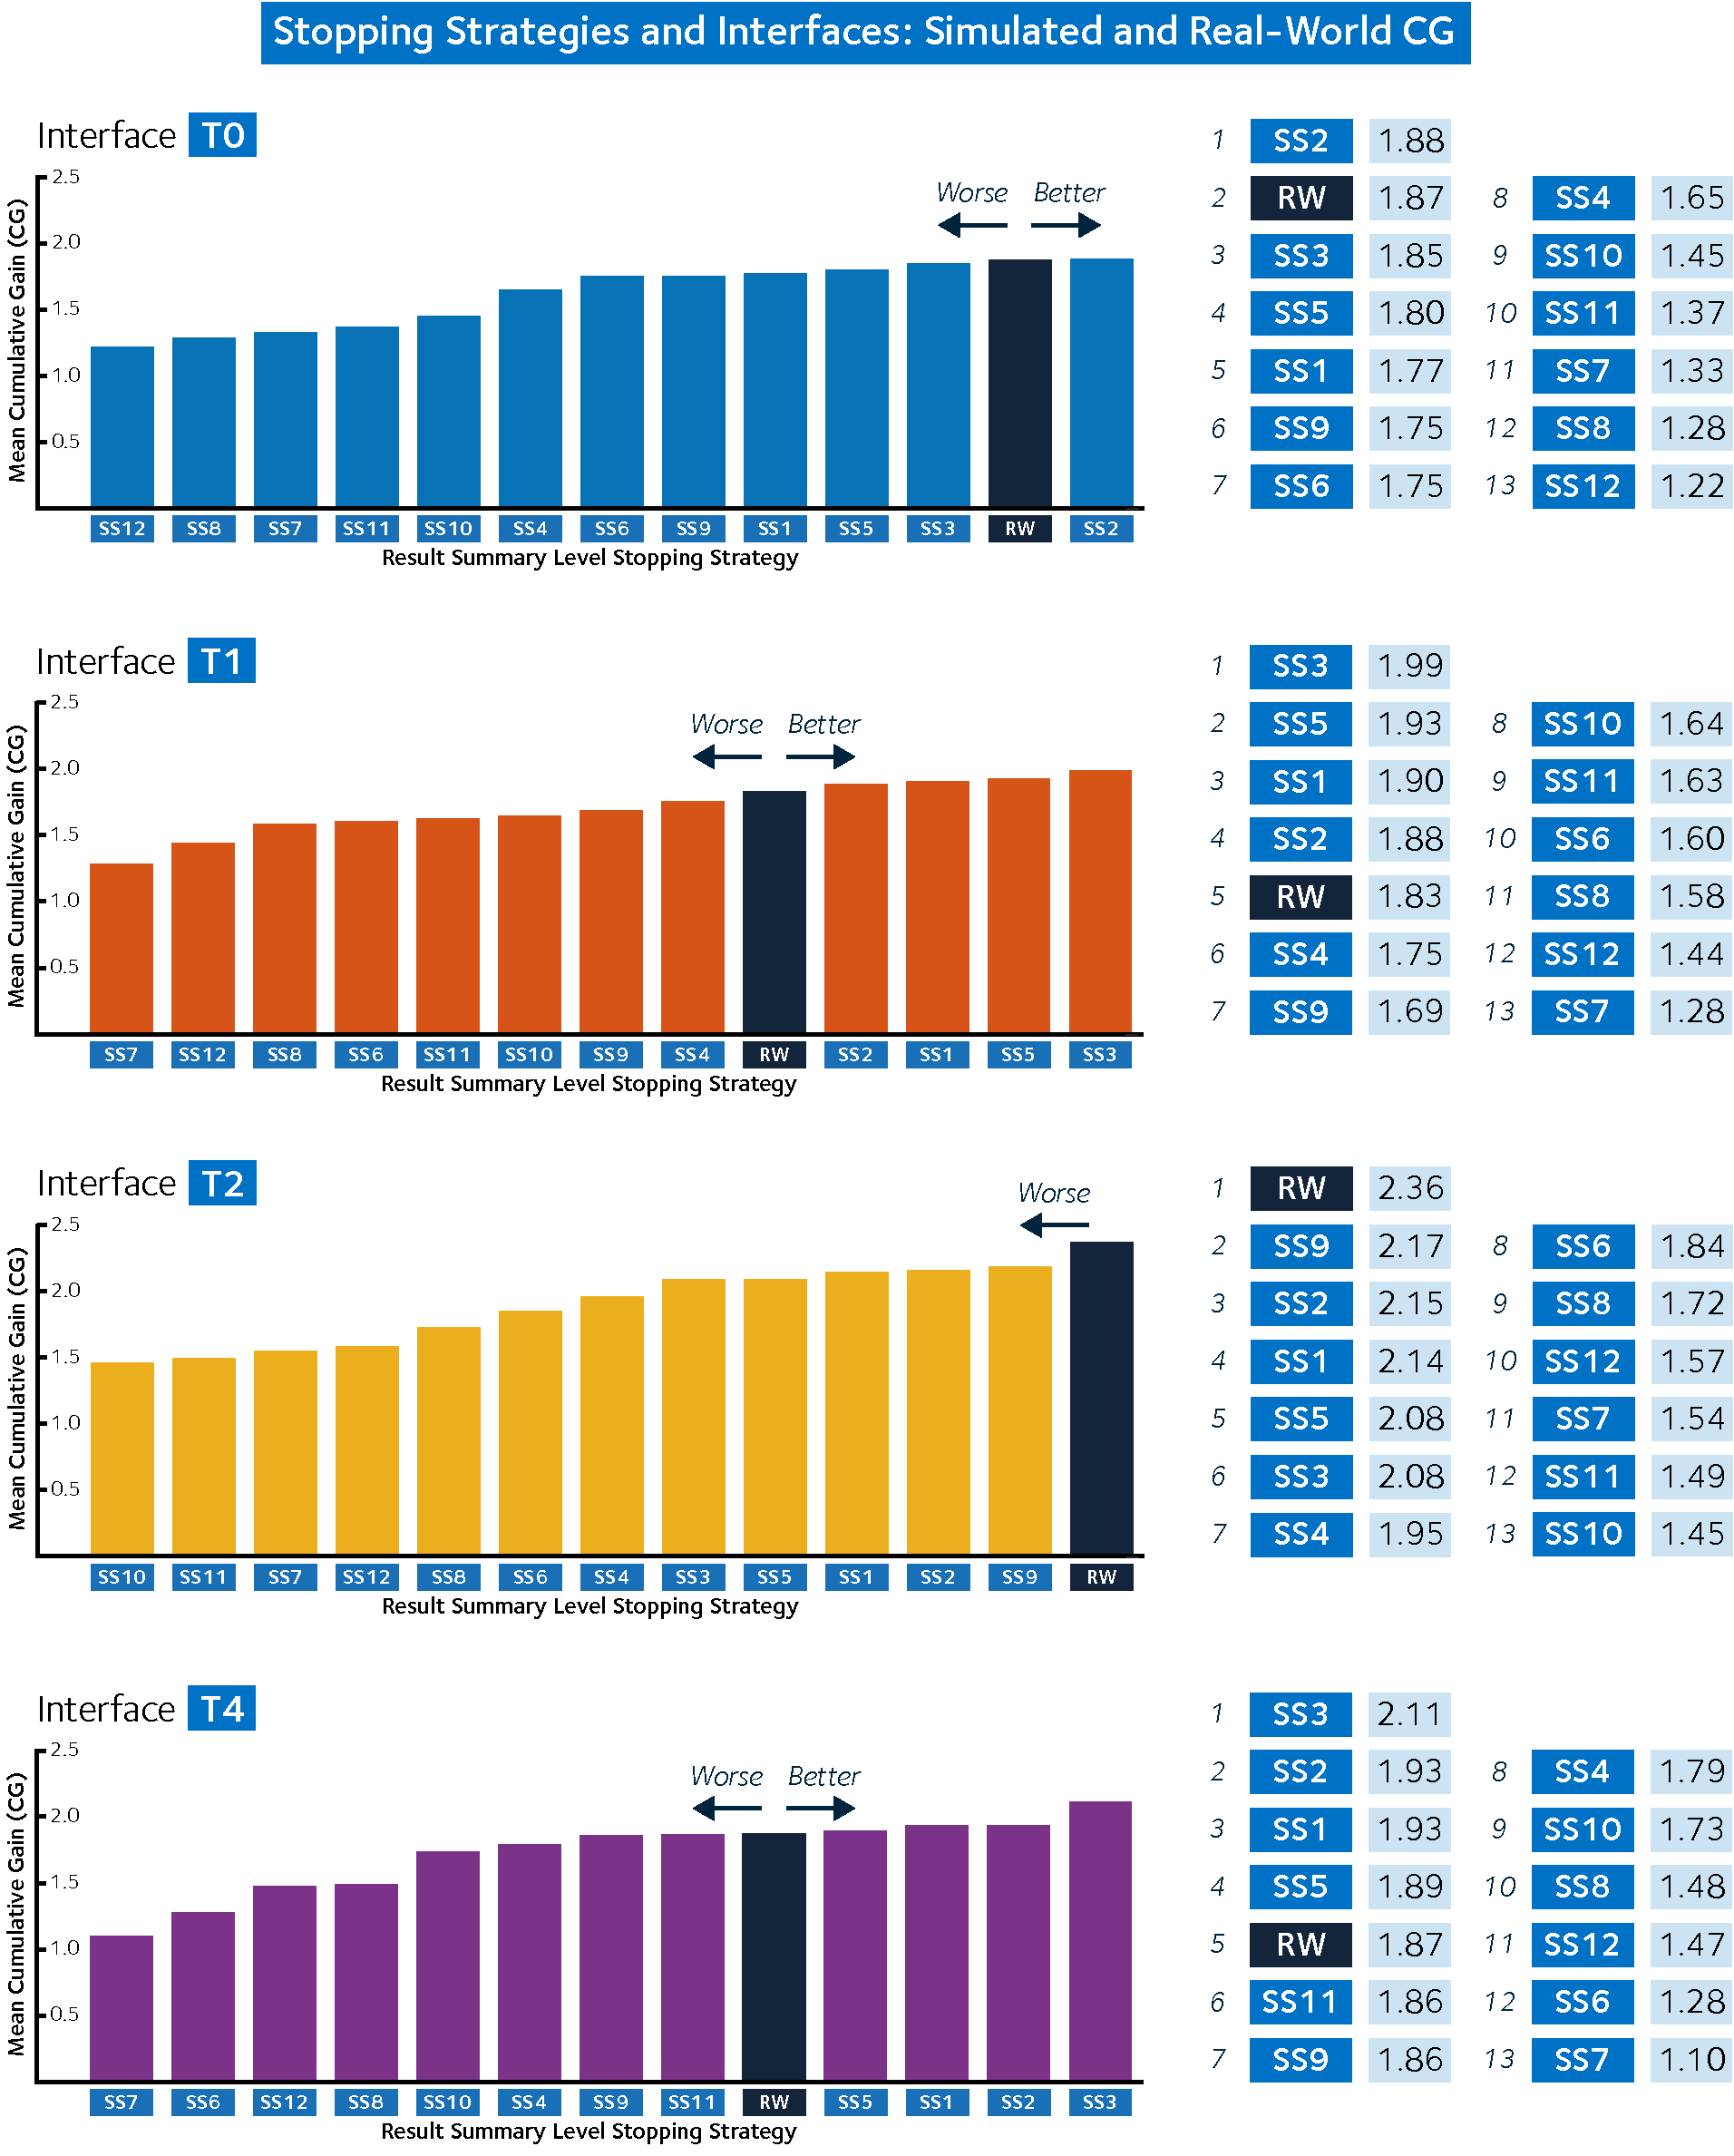
\includegraphics{figures/ch7-comparison_rankings.pdf}}
    \caption[Simulated and real-world~\gls{acr:cg} rankings]{Bar charts, one per experimental interface, demonstrating the mean level of~\gls{acr:cg} attained by each result summary level stopping strategy. Ordered by~\gls{acr:cg}, these values are reached using the threshold configurations yielding the best approximations to actual searcher behaviour, as shown in Table~\ref{tbl:ch7_sim_comp}. Also included are the mean real-world searcher~\gls{acr:cg} values for each interface.}
    \label{fig:ch7_sim_comparison_rankings}
\end{figure}

Stopping strategies offering better approximations also reported a higher mean number of~\gls{acr:trec} relevant documents that were identified (saved). For example, \dualbluebox{SS4-SAT}{@5} over interface \blueboxbold{T2} reported a mean of saved $1.26$~\gls{acr:trec} relevant documents. This is however lower than the real-world mean of $2.47$. Interestingly, we find that stopping strategies \blueboxbold{SS1-FIX}, \blueboxbold{SS2-NT} and \blueboxbold{SS3-NC} all consistently report the highest levels of mean saved~\gls{acr:trec} documents across the four interfaces, albeit still lower than the real-world means. For example, \dualbluebox{SS2-NT}{@21} reports a mean of $1.25$ saved documents over interface \blueboxbold{T0}, compared to $0.89$ over \dualbluebox{SS7-DKL}{@4.0}. This is in contrast to the real-world mean of $1.87$.

Considering the levels of~\gls{acr:cg} attained, we also find some interesting results. The values in Table~\ref{tbl:ch7_sim_comp_cgdq} indicate the level of~\gls{acr:cg} that a searcher would be able to accumulate on average if they rigidly followed a given stopping strategy, using the stopping threshold value(s) that yielded the best approximations. In other words, if rigidly following a given stopping strategy, \emph{would searchers have been able to accumulate higher levels of~\gls{acr:cg} (on average) compared to what they actually achieved?} In order to better represent these results, we generated a series of bar charts, as shown in Figure~\ref{fig:ch7_sim_comparison_rankings}. Each bar chart represents an individual experimental interface; each bar represents the mean level of~\gls{acr:cg} attained over one of the twelve stopping strategies, plus the additional mean real-world~\gls{acr:cg} that was attained.

Results show that on average, real-world searchers typically appear on the high end of the spectrum across all four experimental interfaces. This suggests that given the twelve stopping strategies that were trialled, not many would have offered improvements in overall levels of~\gls{acr:cg}. This is especially true for interface \blueboxbold{T2}, where the real-world~\gls{acr:cg} mean topped all twelve stopping strategies. For interfaces \blueboxbold{T0}, \blueboxbold{T1} and \blueboxbold{T4} where simulations do offer better levels of~\gls{acr:cg}, we find the same stopping strategies appearing above the real-world mean: \blueboxbold{SS1-FIX}, \blueboxbold{SS2-NT}, \blueboxbold{SS3-NC} and \blueboxbold{SS5-COMB}. These results are interesting, as they suggest that a simple stopping strategy is an effective means for attaining high levels of~\gls{acr:cg}, even that of the fixed-depth baseline. Combination stopping strategy \blueboxbold{SS11-COMB} consistently ranked lower across all four interfaces, even though this yielded the highest levels of~\gls{acr:cg} in the performance runs reported in Section~\ref{sec:snippets:simulations:results:perf}.

\section{Chapter Summary}
In this chapter, we have examined how result summary snippet lengths affect a searcher's behaviour, performance and user experience via a crowdsourced user study (Section~\ref{chap:snippets:user}). From this user study, we then subsequently used interaction data from said user study to ground an extensive set of simulations of interaction (Section~\ref{sec:snippets:simulations}). These simulations were trialled to determine how each of the twelve stopping strategies proposed in Chapter~\ref{chap:strategies} performed and approximated the mean stopping behaviours of searchers. In turn, these findings provide answers to our two high-level research questions \darkblueboxbold{HL-RQ3a} and \darkblueboxbold{HL-RQ3b} when varying result summary snippet lengths.

The main finding from the user study showed that as snippet lengths increased across the four experimental interfaces trialled (from interface \blueboxbold{T0} to interface \blueboxbold{T4}), subjects felt that they became more confident with the decisions they were making with respect to identifying relevant material. This can be cited to the fact that more text in the result summary yielded a greater insight into the corresponding document at the cost of greater examination time. A disconnect however existed between how subjects \emph{believed} they performed, and what was actually attained through empirical evidence. Here, we found that as snippet lengths increased, subjects became more \emph{click happy,} marking more documents as relevant, even though accuracy did not improve. This is particularly clear when examining the interaction probabilities that we extracted from interaction data, as reported in Table~\ref{tbl:snippets_probabilities}.

These interaction probabilities (and costs) were then used as a basis for grounding an extensive set of simulations of interaction. Split across performance (addressing \darkblueboxbold{HL-RQ3a}) and comparison runs (addressing \darkblueboxbold{HL-RQ3b}), we examined each individual stopping strategy in both terms of overall performance, and how well they approximated actual searcher stopping behaviours -- all the while across the four experimental interfaces we trialled from the user study. Findings for \darkblueboxbold{HL-RQ3a} show that all twelve stopping strategies offer reasonable levels of~\gls{acr:cg} -- although we found that combination stopping strategy \blueboxbold{SS11-COMB} consistently provided the highest levels of~\gls{acr:cg} across all four experimental interfaces. This was however largely achieved without achieving statistical significance from the remaining eleven strategies. Likewise, for \darkblueboxbold{HL-RQ3b}, we found that \blueboxbold{SS1-FIX} appeared to offer the lowest MSE (and thus best approximations) to actual searcher behaviour, a surprising result. This was largely consistent across interfaces. We also showed that if followed rigidly, several stopping strategies offered improved levels of~\gls{acr:cg} than compared to the real-world mean. No significant differences existed between the stopping strategies. While interesting, these results show that even with slight differences between interfaces in terms of how real-world subjects interacted, there is not a sufficiently large difference between interfaces to affect their stopping behaviours on average in any significant way.

These findings will be considered in detail in Chapter~\ref{chap:conclusions}. Along with the findings of the two remaining empirical contribution chapters, we will consider all of our findings from the stopping strategy simulations in detail, determining what conclusions can be drawn from the this work. Our next chapter considers how altering search tasks and goals affects stopping behaviours -- and whether this is reflected by what stopping strategies perform and approximate best.

\newpage
\thispagestyle{empty}
\mbox{}